%========================================================================
%  RESULTS -- Schreibgeruest
%------------------------------------------------------------------------
%  LESEHILFE (identisch zu evaluation.tex):
%   * "WAS HIER STEHT" = inhaltliche Checkliste, Satz fuer Satz abarbeiten.
%   * "ZAHLEN"         = die bereits VERIFIZIERTEN Werte aus dem Run.
%                        Alle Zahlen unten wurden direkt aus den Tabellen
%                        gelesen -- du musst nichts nachrechnen, aber du
%                        darfst auch KEINE Zahl schreiben, die hier nicht
%                        steht (CLAUDE.md Rigor-Regel).
%   * "ZITATE"         = biblatex-Keys (alle bereits in references.bib).
%   * "!! ENTSCHEIDUNG"= Punkt, den DU faellen musst; ich habe ihn bewusst
%                        offen gelassen (meist Coverage-vs-Winkler).
%   * "[arXiv-Kuerzung]" = wie das Unterkapitel fuer arXiv eingedampft wird.
%   * Bloecke zwischen % >>> THESIS-ONLY >>> und % <<< THESIS-ONLY <<<
%                        fliegen fuer arXiv komplett raus.
%
%  DATENHERKUNFT ALLER ZAHLEN IN DIESER DATEI
%  ------------------------------------------
%  Diagnostics-Run : run_full_20260803_095330   (03.08.2026, mode=full)
%  Conformal-Run   : run_full_20260721_145309
%  Modell-Runs     : rw/arma/tirex/lgbm 21.07. 12:54--12:57,
%                    xlstm 13:23, lstm 13:55, tirex2 14:14
%  Panel-Hash      : data_sha256 5f27a412...68ec2e  (IDENTISCH ueber alle
%                    sieben Modellfamilien -> alle Modelle sahen dasselbe
%                    33d-TARGET2-Panel. Das ist der Beleg, dass der Rebuild
%                    sauber durchgezogen wurde -- unbedingt EINMAL im Text
%                    erwaehnen, das ist ein Reproduzierbarkeits-Argument.)
%  git commit      : b1811e67b6a92460cdf94e405d29093a5945680f
%  Kopien der Tabellen liegen im Repo unter  results/tables/*.csv
%  Story-Report (autom. Findings) unter      results/story_report.md
%
%  GRUNDGEROESSEN DES RUNS (in 8.1 nennen, danach nie wieder)
%   Testfenster        : 127 Monate, 2015-10 bis 2026-04
%   Laender            : 10
%   Kombinationen      : 742  (Modell x Regime x Seed x CP-Methode)
%   Zellen             : 21200 (davon 7420 im Primaer-Pool "rolling")
%   Kontraste          : 1249 vorregistriert + 66 post-hoc (XM)
%   Findings           : 816
%   Modelle            : 12 (6 Basis + 3 const-width-Twins + arma_monthly
%                            + tirex + tirex2_cov)
%   Regime             : L, G, GF, GI, ZS
%   CP-Methoden        : 14
%   Seeds              : 42, 43, 44 (nur NN)
%   alpha=0.20, FDR q=0.10, Gate-Schwelle 70%, MCS alpha=0.10,
%   Block-Bootstrap 6/1000, DQ-Lags 4, Rolling-Coverage-Fenster 36
%========================================================================
\section{Results}
\label{sec:results}
We evaluate 742 combinations (Modell x Regime x Seed x CP-Methode) over 127 Months and 10 countries with all Models run on the same panel of data ($data\_sha256$). First we discuss the Gating that decides wether we evaluate a combination further, then the results of the point forecasting followed by the intervall ranking. Next the findings regarding the research questions are beeing classified, the impact the covariates and Regimes on the outcome acesssed. The winners of the Cross Model MCS acessed will be announced and finaly we will discuss the robustness of the results. Since we are using the winkler score as our main scoring mechanism a lower score means better and negative d norm means one model is performing better than the other. A positive skill means the Model performed better than the reference model (Random walk with native quintiles). 
% WAS HIER STEHT (Kapitel-Kopf, 1 Absatz, KEINE Zahlen ausser den Groessen):
%  - Ein Satz: was ausgewertet wird (742 Kombinationen auf 127 Testmonaten
%    x 10 Laendern), und dass alle Modellfamilien auf demselben Panel
%    liefen (data_sha256 identisch).
%  - Ein Satz Leseanleitung: erst das Gate (8.1), dann Punktprognose (8.2),
%    dann das Intervall-Ranking (8.3), dann die drei vorregistrierten
%    Forschungsfragen (8.4-8.6), dann Kovariaten (8.7), Cross-Model+MCS
%    (8.8), Regime (8.9), Oekonomie (8.10), Robustheit (8.11).
%  - Ein Satz zur Lesekonvention: negative d_norm bedeutet A besser als B
%    (Winkler ist ein Verlust); Skill > 0 bedeutet besser als RW/L/native.
%    -> Das MUSS einmal explizit dastehen, sonst liest der Leser jede
%       Kontrasttabelle falsch herum.
%
% [arXiv-Kuerzung]: bleibt, auf 3 Saetze.


%------------------------------------------------------------------------
\subsection{The evaluation universe and the validity gate}
\label{sec:res:gate}
%------------------------------------------------------------------------
We are working with 742 combinations on 127 Test months over 10 countries. Only 65,4 percent of all combinations (485) suvived the validity Gate. We see that the Gate is no formalism, it sorts out about a third of all combinations. \\
As we see in the table the nativ models have difficulties passing the gate. This is due to the fact that they are very conservative with an average coverage of 0.872 instead of 0.8. The Problem is solved by the various conformal methods. Greece and Portugal have with respectively 0.519 and 0.616 the lowest acceptance rates. France (0.864) and Finland (0.844) have the highest acceptance rates. This shows that the prediction intervalls for the spreads of the periphery countries are harder to calibrate. The Gate only uses the Kupiec and Christoffersen test the DQ Test that additionaly tests for 4 lags and with rejects 49.3$\%$ of all cobinations (q<0.10) \cref{sec:res:limitations}. This shows that Conditional calibrations is violated even in combinations that pass the Gate \cite{kupiec1995, christoffersen1998, engle2004caviar, benjamini1995fdr}.\\
Quantile crossing occurs when the model output for the lower bound is higher than the one for the higher bound. For us it occurs in 0.451$\%$ of predictions and in $0.398\%$ of predictions from accepted combinations. $81.7\%$ of combinations never produce quantile crossing, with native and $saocp\_cqr$ having $0\%$ \cref{sec:conformal:notes}.
$pid\_tan\_cqr$ has, with $2.554\%$, the highest crossing rate. $cqr\_static$ has $0.724\%$ \cref{sec:res:ranking} crossing rate but in extreme cases (xlstm/L/seed42/IE) up to $77.95\%$. 18 out of $cqr\_static$ cells have above $5\%$ crossing rate.
Crossing is on average negligible, but not equality distributed
% WAS HIER STEHT:
%  1. Groessen des Auswertungsraums nennen (Liste oben im Kopfkommentar).
%  2. Das ERGEBNIS DES GATES als erste substanzielle Aussage:
%     485 von 742 Kombinationen (65.4%) sind admissible.
%     -> Der Satz, der hier hingehoert: das Gate ist kein Formalismus,
%        es sortiert ein gutes Drittel des Suchraums aus.
%  3. Die Gate-Rate NACH CP-METHODE ist die eigentliche Story dieses
%     Unterkapitels: sie zeigt, dass "native" als Intervallquelle fast
%     immer fehlkalibriert ist und die CP-Schicht das repariert.
%     -> Das ist auch schon die halbe Antwort auf RQ3 (8.4). Hier nur
%        deskriptiv, die Inferenz kommt in 8.4.
%  4. Ein Satz zur Richtung der Fehlkalibrierung: es ist UEBERdeckung,
%     nicht Unterdeckung. native-Coverage im Mittel 0.872 statt 0.80.
%     Das ist wichtig fuers Framing: die Modelle sind nicht "zu optimistisch",
%     sie sind zu konservativ -> Intervalle unnoetig breit -> teuer
%     (Anschluss an 8.10 Kapital-Proxy).
%  5. Gate-Rate nach LAND: GR (0.519) und PT (0.616) am schwersten,
%     FR (0.864) und FI (0.844) am leichtesten. Ein Satz Interpretation:
%     die Peripherie mit sprunghaften Spreads ist am schwersten kalibrierbar.
%  6. Ein Satz Ehrlichkeit (WICHTIG, sonst Referee-Angriff): das Gate
%     benutzt nur Kupiec+Christoffersen. Der DQ-Test, der zusaetzlich auf
%     Breite und 4 Lags konditioniert, verwirft in 49.3% aller Zellen
%     (q<0.10). Bedingte Kalibrierung ist also breitflaechig verletzt,
%     auch bei Kombinationen, die das Gate passieren. Das MUSS hier stehen
%     und in 8.12/Limitations wiederholt werden.
%     -> AUSGEBAUT 2026-08-03: die Zerlegung dieser 49.3% (es ist fast
%        vollstaendig der BREITEN-Regressor, nicht die Lags) steht im
%        Limitations-Block L1 am Ende dieser Datei. Hier nur die Zahl und
%        einen Vorwaertsverweis setzen -- die Erklaerung gehoert nicht in
%        den deskriptiven Teil.
%  7. QUANTILKREUZUNG -- NEU EINZUFUEGEN 2026-08-03. Wird in
%     \cref{sec:conformal:notes} als Mechanismus beschrieben ("in rare
%     cases the calibrated interval inverts"), aber im Ergebnisteil nie
%     quantifiziert. Zwei Saetze genuegen, und sie schuetzen dich gegen
%     einen Standard-Angriff auf Quantilregression.
%     ZAHLEN (cells.csv, Spalte crossed_cal_rate, pool=rolling):
%       Gesamtmittel 0.451% | nur zulaessige Kombis 0.398%
%       81.7% aller Zellen kreuzen NIE
%       native und saocp_cqr: exakt 0.000% (bei native per Konstruktion,
%         bei saocp wegen der nichtnegativen Radien -- das bestaetigt die
%         in \cref{sec:conformal:notes} Punkt 2 behauptete
%         Domaeneneigenschaft empirisch, ein Satz wert)
%       pid_tan_cqr 2.554% -- eine Groessenordnung ueber dem Feld
%       cqr_static 0.724% im Mittel, aber mit Extremfaellen bis 77.95%
%         (xlstm/L/seed42/IE); 18 von 530 cqr_static-Zellen ueber 5%
%     -> DER SATZ, DER HIER HINGEHOERT: Kreuzung ist im Mittel
%        vernachlaessigbar, aber sie ist nicht gleichverteilt, und sie
%        trifft ausgerechnet cqr_static -- die Methode des
%        Spitzenreiters. tirex2/ZS/cqr_static hat in PT eine
%        Kreuzungsrate von 32.3%. Das ist ein weiteres Argument in der
%        Entscheidung unter 8.3 Punkt 4 und sollte dort verlinkt werden.
%        (decay_ocp_cqr zum Vergleich: 0.028%.)
%
% ZAHLEN (verifiziert):
%   Gate gesamt          : 485/742 valide  (= 65.4%)
%   Gate-Rate je CP-Methode (validity_flags.csv / ranking_all.csv):
%       dtaci_cqr 1.000 | pid_cqr 1.000 | pid_local_cqr 1.000
%       sfogd_cqr 1.000 | spci_cqr 1.000 | agaci_cqr 0.981
%       aci_cqr 0.962   | cqr_rolling 0.906 | mondrian_cqr 0.604
%       pid_tan_cqr 0.283 | decay_ocp_cqr 0.208 | native 0.132
%       cqr_static 0.057 | saocp_cqr 0.019
%   Mittlere Coverage je Methode (cells.csv, pool=rolling, alle Zellen):
%       spci 0.769 | sfogd 0.806 | agaci 0.811 | pid 0.813 | pid_local 0.814
%       aci 0.815 | dtaci 0.822 | cqr_rolling 0.823 | pid_tan 0.824
%       cqr_static 0.859 | mondrian 0.860 | native 0.872 | decay_ocp 0.873
%       saocp 0.917
%       -> Zielwert ist 0.80. native = +7.2pp, saocp = +11.7pp Ueberdeckung.
%   Gate-Rate je Modellfamilie: tirex2 0.857 | tirex2_cov 0.857 |
%       tirex 0.786 | lgbm 0.714 | arma 0.714 | arma_monthly 0.714 |
%       lgbm_const 0.679 | lstm_const 0.659 | rw 0.643 | xlstm_const 0.643 |
%       lstm 0.625 | xlstm 0.613
%   Gate-Rate je Regime: ZS 0.833 | L 0.668 | G 0.643 | GF 0.631 | GI 0.602
%   Gate-Rate je Land (calibration_tests.csv, cell_valid):
%       FR 0.864 | FI 0.844 | IT 0.810 | NL 0.771 | AT 0.747 | BE 0.718
%       ES 0.660 | IE 0.623 | PT 0.616 | GR 0.519
%   Rohe Ablehnraten ueber alle 7420 Zellen (calibration_tests.csv):
%       UC : p<0.05 23.4% -> q<0.10 20.6%
%       IND: p<0.05 16.2% -> q<0.10  6.1%
%       CC : p<0.05 31.0% -> q<0.10 26.3%
%       DQ : p<0.05 49.6% -> q<0.10 49.3%
%   DQ-Ablehnrate je Methode (Auswahl): mondrian 0.291, dtaci 0.300,
%       pid 0.304, agaci 0.345, cqr_rolling 0.368, aci 0.377, ...,
%       native 0.562, cqr_static 0.617, sfogd 0.632, spci 0.666,
%       pid_tan 0.938
%
% TABELLE: tab:res_gate unten -- Zahlen sind schon eingetragen, du
%   schreibst nur die Caption + den Fliesstext drumherum.
%
% ZITATE: kupiec1995, christoffersen1998, engle2004caviar, benjamini1995fdr.
%
% [arXiv-Kuerzung]: 1 Absatz + tab:res_gate. Der Laender-Schnitt und die
%   Regime-Gate-Raten fliegen raus.

\begin{table}[t]
\centering
\caption{% TODO Caption. Inhalt: Gate-Durchfallquote und mittlere Coverage
         je Rekalibrierungsmethode. Zielcoverage 0.80.}
\label{tab:res_gate}
\begin{tabular}{lccc}
\toprule
Method & Admissible share & Mean coverage & DQ rejection rate \\
\midrule
\texttt{dtaci\_cqr}      & 1.000 & 0.822 & 0.300 \\
\texttt{pid\_cqr}        & 1.000 & 0.813 & 0.304 \\
\texttt{pid\_local\_cqr} & 1.000 & 0.814 & 0.458 \\
\texttt{sfogd\_cqr}      & 1.000 & 0.806 & 0.632 \\
\texttt{spci\_cqr}       & 1.000 & 0.769 & 0.666 \\
\texttt{agaci\_cqr}      & 0.981 & 0.811 & 0.345 \\
\texttt{aci\_cqr}        & 0.962 & 0.815 & 0.377 \\
\texttt{cqr\_rolling}    & 0.906 & 0.823 & 0.368 \\
\texttt{mondrian\_cqr}   & 0.604 & 0.860 & 0.291 \\
\texttt{pid\_tan\_cqr}   & 0.283 & 0.824 & 0.938 \\
\texttt{decay\_ocp\_cqr} & 0.208 & 0.873 & 0.525 \\
\texttt{native}          & 0.132 & 0.872 & 0.562 \\
\texttt{cqr\_static}     & 0.057 & 0.859 & 0.617 \\
\texttt{saocp\_cqr}      & 0.019 & 0.917 & 0.523 \\
\bottomrule
\end{tabular}
\end{table}


%------------------------------------------------------------------------
\subsection{Point forecasts: nothing beats the random walk}
\label{sec:res:point}
%------------------------------------------------------------------------
Only TiRex2 beats the random walk with an advantage of $0.35\%$, as can be seen in Table ~\ref{tab:res_point}. All the Models that were trained on the task performed worse than the random walk: xlstm 1.104, $xlstm\_const$ 1.093, lstm 1.061, lgbm 1.065. This leads to the conclusion that the effort of training a Model for point forecasting in this case is not worth the effort. The Models predict the right direction on average in 0.5397$\%$ with the Pesaran Timmermann Test beeing signifacnt at $5\%$ in $7.2\%$ of cells only. This shows that there is no relevant dicational gained from the Models. A forecast is counted as positive if the future value is predicted to be bigger that the current one. Since the random walk always predicts no change it produces negative predictions only and by that is an indicator of how often, percentage wise, the spread went down. The distinction of the Models happens in the next chapter when we talk about, when we talk about uncertainty quantification
% WAS HIER STEHT:
%  Dieses Unterkapitel ist strategisch wichtig: es raeumt die Erwartung ab,
%  dass es hier um bessere PUNKTprognosen geht, und macht damit den Weg
%  frei fuer die eigentliche Botschaft (Intervalle). Es ist ein NEGATIVES
%  Ergebnis und genau deshalb glaubwuerdig -- nicht verstecken, sondern
%  als bewusstes Framing an den Anfang stellen.
%  1. MAE-Ratio-Tabelle: NUR tirex2 liegt unter 1 (0.9965), und das ist
%     ein Vorsprung von 0.35% -- praktisch nicht existent.
%  2. Alle trainierten Modelle sind SCHLECHTER als der Random Walk:
%     xlstm 1.104, xlstm_const 1.093, lstm 1.061, lgbm 1.065.
%     -> Ein Satz: der Aufwand des Trainings zahlt sich auf der
%        Punktprognose nicht aus.
%  3. Richtungsprognose: mittlere Trefferquote 0.540 ueber alle Zellen,
%     der Pesaran--Timmermann-Test ist nur in 7.2% der Zellen auf 5%
%     signifikant. -> Ein Satz: es gibt praktisch keine ausbeutbare
%     Richtungsinformation. (Nominal wuerde man bei reinem Zufall 5%
%     signifikante Tests erwarten -- 7.2% ist kaum mehr. Diesen Vergleich
%     unbedingt hinschreiben, das ist die ehrliche Lesart.)
%  4. Kurioses, aber ehrliches Detail: der Random Walk hat die HOECHSTE
%     Richtungstrefferquote (0.578) -- trivial, weil die RW-Delta-Prognose
%     konstant null ist und die Vorzeichenkonvention ihm das schenkt.
%     !! Pruefe im Code kurz nach, wie dir_acc bei konstant-null-Delta
%        definiert ist, bevor du das interpretierst. Wenn die Konvention
%        "Vorzeichen 0 zaehlt als Treffer" ist, ist die Zahl ein Artefakt
%        und du solltest sie als solches benennen statt sie zu deuten.
%  5. Schlusssatz, der zu 8.3 ueberleitet: die gesamte Differenzierung
%     zwischen den Modellen findet in der Unsicherheitsquantifizierung
%     statt, nicht im bedingten Erwartungswert.
%
% ZAHLEN (verifiziert, cells.csv pool=rolling, Median ueber Laender):
%   Modell        MAE-Ratio  RMSE-Ratio  dir_acc  PT p<0.05
%   tirex2          0.9965     0.9993     0.555     0.100
%   tirex2_cov      1.0008     0.9997     0.534     0.200
%   rw              1.0000     1.0000     0.578     0.000
%   arma_monthly    1.0137     1.0166     0.539     0.200
%   arma            1.0174     1.0166     0.536     0.200
%   tirex           1.0202     1.0168     0.539     0.100
%   lgbm_const      1.0572     1.0406     0.536     0.050
%   lgbm            1.0649     1.0441     0.535     0.033
%   lstm            1.0614     1.0549     0.552     0.075
%   lstm_const      1.0671     1.0565     0.555     0.078
%   xlstm_const     1.0935     1.0744     0.530     0.056
%   xlstm           1.1039     1.0801     0.522     0.058
%   Gesamt: mean dir_acc 0.5397, Anteil PT p<0.05 = 7.2%
%
% ZITATE: pesaran1992, hyndman2006mase (skalenfreie Fehlermasse),
%   dieboldmariano1995 optional.
%
% [arXiv-Kuerzung]: 3 Saetze + tab:res_point. PT-Details in eine Fussnote.

\begin{table}[t]
\centering
\caption{% TODO Caption. Point-forecast accuracy relative to the random
         walk; ratios below one indicate an improvement.}
\label{tab:res_point}
\begin{tabular}{lcccc}
\toprule
Model & MAE ratio & RMSE ratio & Directional accuracy & PT rejections \\
\midrule
\texttt{tirex2}       & 0.997 & 0.999 & 0.555 & 0.10 \\
\texttt{rw}           & 1.000 & 1.000 & 0.578 & 0.00 \\
\texttt{tirex2\_cov}  & 1.001 & 1.000 & 0.534 & 0.20 \\
\texttt{arma\_monthly}& 1.014 & 1.017 & 0.539 & 0.20 \\
\texttt{arma}         & 1.017 & 1.017 & 0.536 & 0.20 \\
\texttt{tirex}        & 1.020 & 1.017 & 0.539 & 0.10 \\
\texttt{lgbm\_const}  & 1.057 & 1.041 & 0.536 & 0.05 \\
\texttt{lstm}         & 1.061 & 1.055 & 0.552 & 0.08 \\
\texttt{lgbm}         & 1.065 & 1.044 & 0.535 & 0.03 \\
\texttt{lstm\_const}  & 1.067 & 1.057 & 0.555 & 0.08 \\
\texttt{xlstm\_const} & 1.093 & 1.074 & 0.530 & 0.06 \\
\texttt{xlstm}        & 1.104 & 1.080 & 0.522 & 0.06 \\
\bottomrule
\end{tabular}
\end{table}


%------------------------------------------------------------------------
\subsection{Main ranking: interval skill}
\label{sec:res:ranking}
%------------------------------------------------------------------------
The Table ~\ref{tab:res_ranking} ranks the best perfroming (winkler skill) calibrations per model famly. As we can see the best Performing Modell is $tirex2/ZS/cqr\_static$ followed by $tirex2\_cov/ZS/native$ with respective median winkler skills of $0.146$/ $0.141$ and mean coverage of $0.75/0.839$. With both beeing admissible in only 8/10 countries. The best two valid Models are zero shot foundation models that wasnt trained on the data during this study.\\ 
The first model that has been trained by ourselfes is $lgbm/G/decay\_ocp\_cqr$, it is ranked third, with a median winkler skill of $0.139$ and mean coverage of $0.824$. The best classical approach $rw/L/aci\_cqr$ reached 8th place with a median winkler skill of $0.085$, mean coverage of $0.812$ and beeing admissable in all 10 countries. The same Model that is equal at point forecasting to the random walk beats it at producing prediction intervalls. This leads us to the conclusion that the advantage of the Model is soley in the predicting the distribution not the center. The xLSTM familie turned out to be the wort perfroming with a median skill over all combinations of $-0.047$.The best valid combination of the Familie is $xlstm/L/native$ with $0.094$ and without usage of the CP layer. In the GI regime we also see a negative skill of $-0.042$.\\

In Table ~\ref{tab:res_tirex2_cp} we take a closer look at the winning Model family tirex2/ZS. We see that the second best performing (winkler skill) CP method $decay\_ocp\_cqr$ only has a difference, in winkler skill, of 0.002 to the elading Model but its coverage (0.787) is way closer to the target of 0.8 and its admissable in all 10 countries. Inside this familie the Median skill reaches from $-0.044$ $(pid\_tan)$ up to $0.146$ $(cqr\_static)$. We conclude that the choice of the calibration method is as important to the outcome as the choice of the underlying Model.
\begin{figure}[htbp]
    \centering
    \makebox[\textwidth][c]{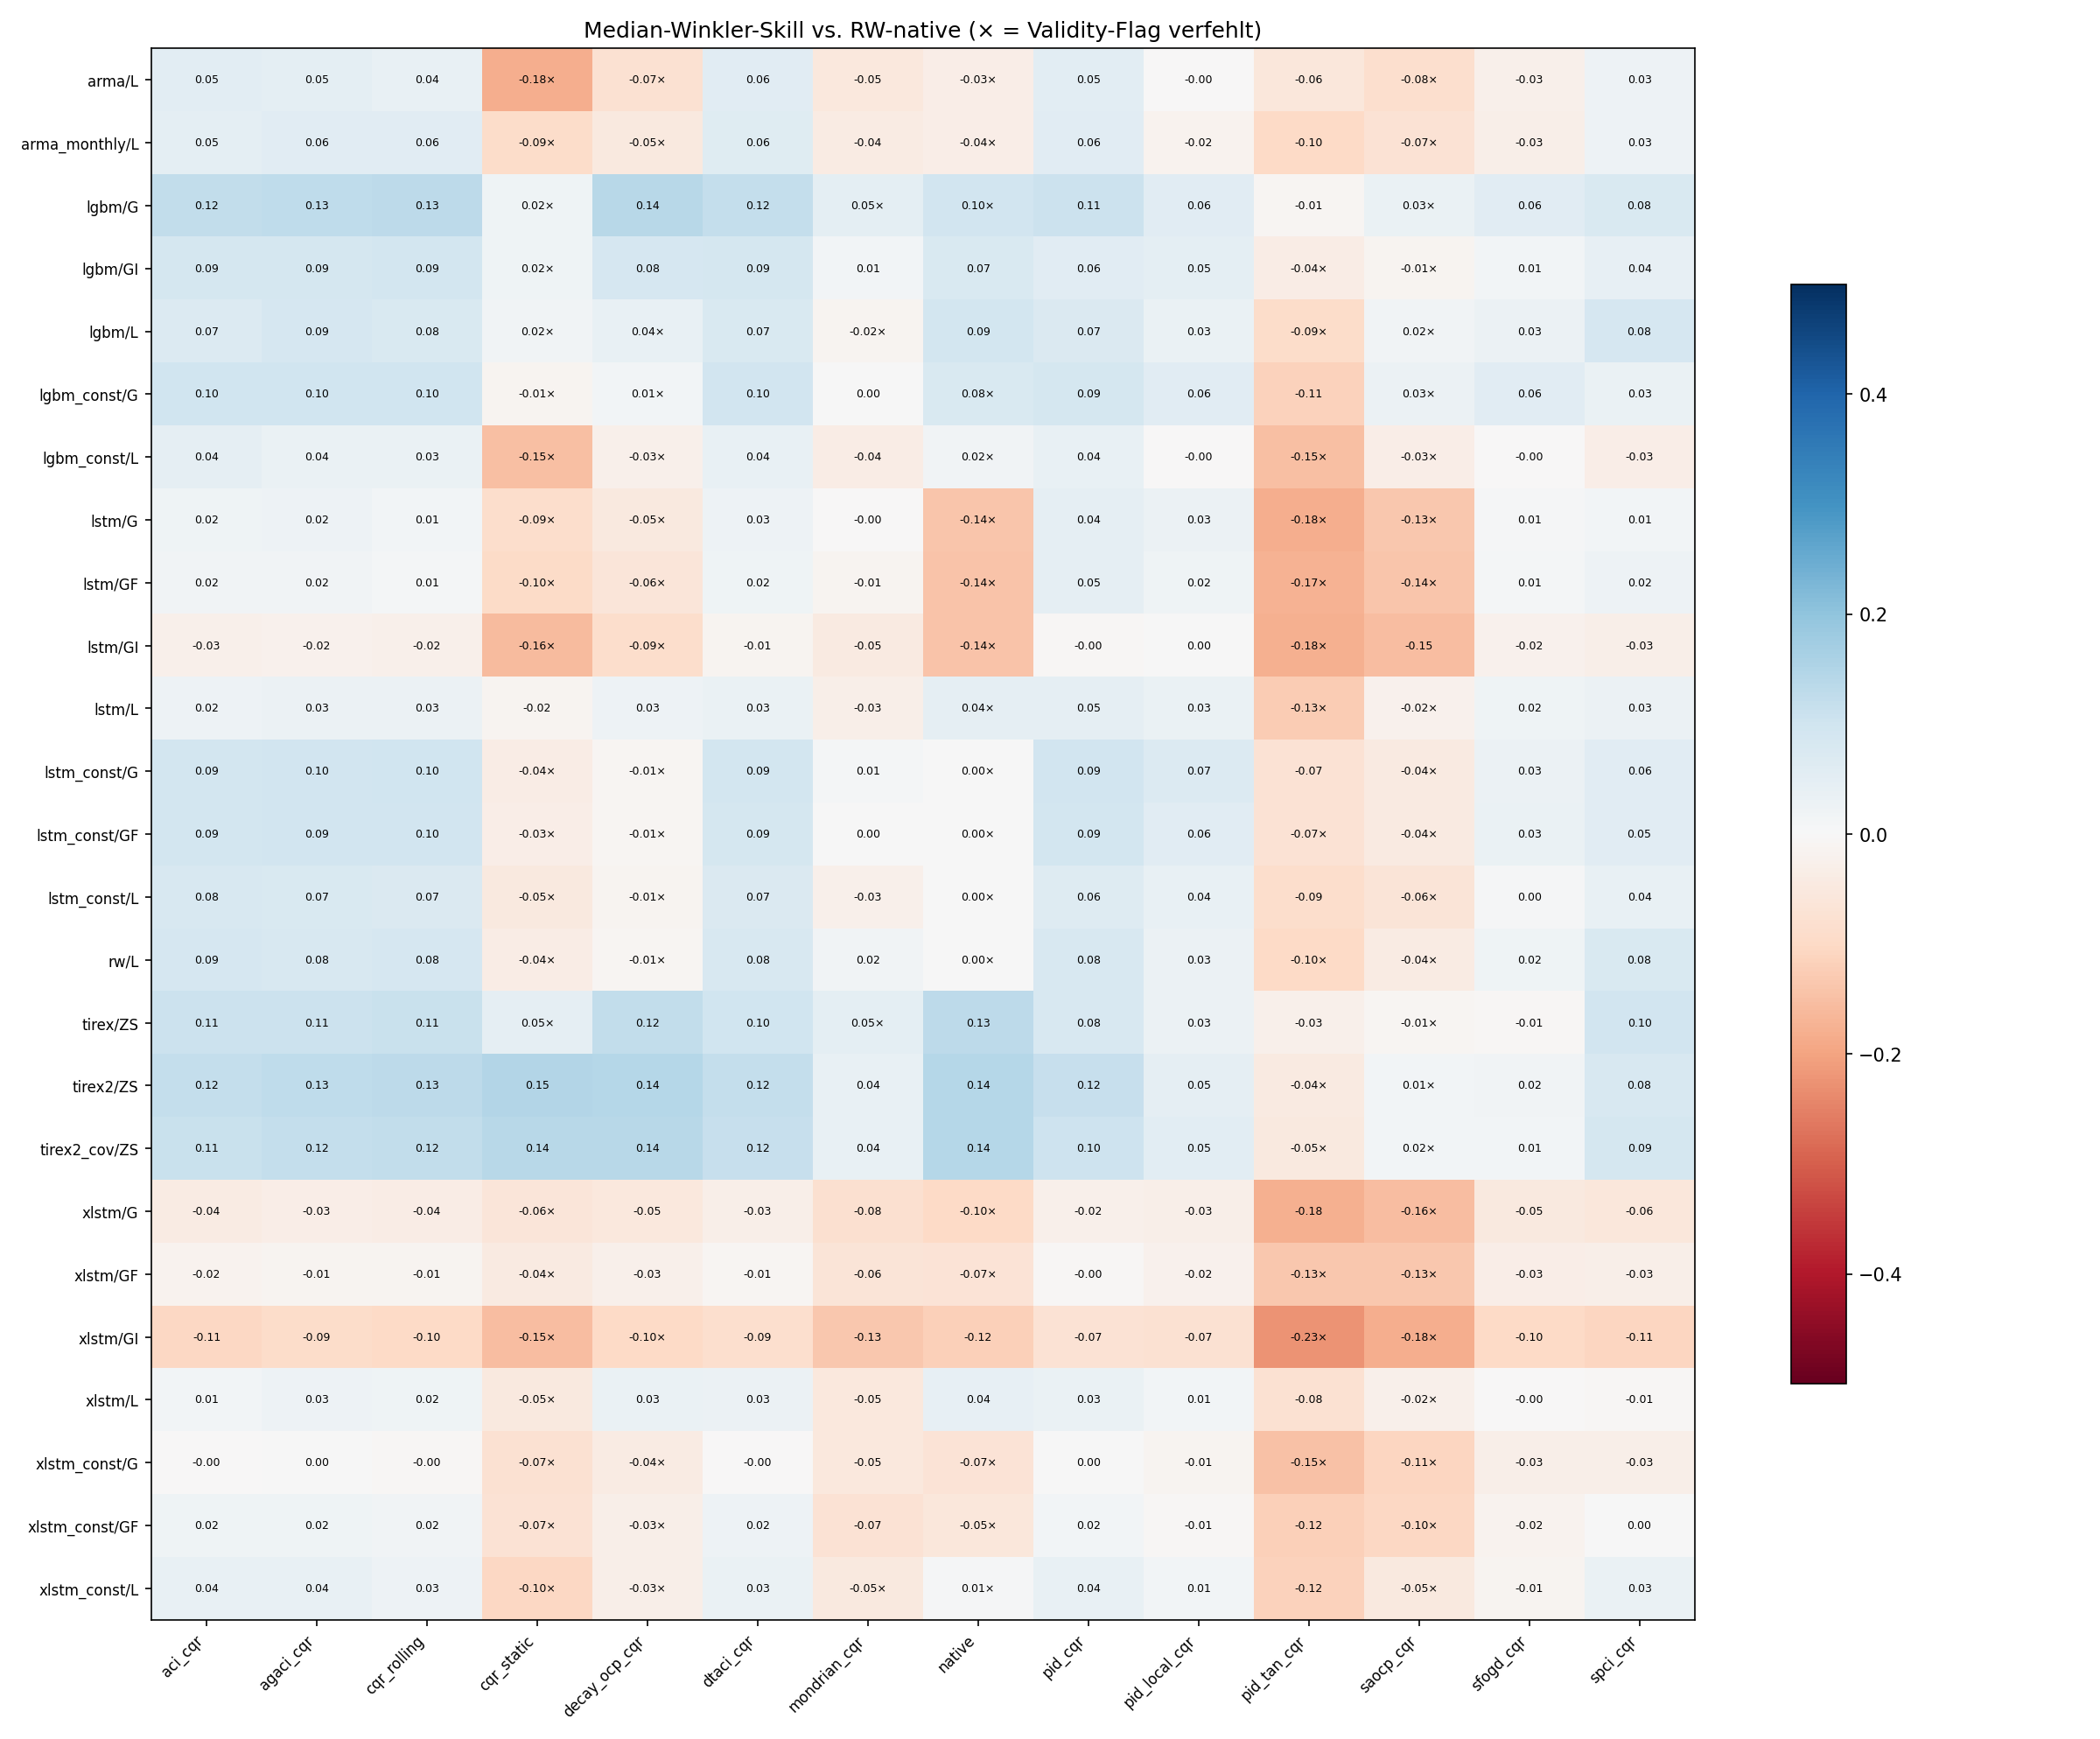
\includegraphics[width=1.15\textwidth]{figures/skill_heatmap.png}}
    \caption{Heatmap zur Übersicht der Modell-Skills.}
    \label{fig:skill_heatmap}
\end{figure}

% Das ist DAS Kernunterkapitel der Arbeit. Nimm dir hier am meisten Zeit.
%
% WAS HIER STEHT:
%  1. Das Ranking der besten validen Kombination je Modellfamilie
%     (tab:res_ranking unten, Zahlen eingetragen).
%  2. Die Kernaussage: das beste valide Paket ist ein ZERO-SHOT-
%     Foundation-Model ohne jedes Training auf diesen Daten
%     (tirex2/ZS), mit Winkler-Skill 0.146 gegen RW/L/native. Der beste
%     klassische Ansatz (rw/L/aci_cqr) kommt auf 0.085.
%     -> Ein Satz, der die Spannung benennt: dasselbe Modell, das bei der
%        Punktprognose exakt auf RW-Niveau liegt (8.2), erzeugt die mit
%        Abstand besten Intervalle. Der Vorsprung liegt vollstaendig in
%        der Form der praediktiven Verteilung, nicht in ihrem Zentrum.
%  3. Das xLSTM-Ergebnis EHRLICH aufschreiben. Das ist die namensgebende
%     Architektur der Arbeit und sie ist die SCHWAECHSTE Familie:
%     Median-Skill ueber alle Kombis -0.047 (letzter Platz), bestes
%     valides Paket xlstm/L/native mit 0.094 -- und das ausgerechnet mit
%     der nativen Quantilausgabe, also OHNE Nutzen aus der CP-Schicht.
%     Im GI-Regime ist der Skill negativ (-0.042).
%     -> Das nicht kleinreden. Ein negatives Kernergebnis, das sauber
%        gemessen wurde, ist wissenschaftlich wertvoller als ein
%        herbeigeredetes positives. In der Discussion aufgreifen:
%        277 Monate x 10 Laender sind schlicht zu wenig Daten fuer eine
%        Architektur dieser Kapazitaet.
%  4. !! ENTSCHEIDUNG -- COVERAGE VS. WINKLER (CLAUDE.md verbietet mir,
%     das fuer dich zu entscheiden):
%     Der Spitzenreiter tirex2/ZS/cqr_static hat Skill 0.1461, aber
%     mittlere Coverage 0.7496 -- also 5.0pp UNTER dem Ziel von 0.80 --
%     und passiert das Gate nur in 8 von 10 Laendern.
%     Der direkte Verfolger tirex2/ZS/decay_ocp_cqr hat Skill 0.1442
%     (0.0019 weniger, also 1.3% relativer Unterschied), aber Coverage
%     0.7866 und ist in 10 von 10 Laendern valide; mittlerer absoluter
%     Coverage-Abstand zum Ziel: 0.0279 gegenueber 0.0680 bei cqr_static.
%     DREI moegliche Auflösungen -- waehle EINE und begruende sie:
%       (a) cqr_static als Headline, decay_ocp als robustere Alternative
%           nennen. Maximiert die Schlagzeile, laedt aber den Vorwurf ein,
%           dass der Sieger unterdeckt.
%       (b) decay_ocp als Headline (Coverage-naeher, 100% Gate), cqr_static
%           als "hoechster Rohskill" in einem Nebensatz. Konservativ,
%           konsistent mit dem validity-first-Prinzip aus 7.1.
%       (c) Beide gemeinsam als "tirex2/ZS-Familie, Skill 0.14-0.15"
%           berichten und die Methodenwahl explizit als offen deklarieren.
%     MEINE EMPFEHLUNG: (b). Begruendung: du hast in 7.1 validity-first
%     als tragendes Prinzip vorregistriert. Wenn du dann die Kombination
%     mit dem groessten Coverage-Fehler zum Sieger kuerst, untergraebst du
%     dein eigenes Kriterium, und genau das wird ein Referee angreifen.
%     Aber es ist DEINE Entscheidung -- schreib sie explizit hin.

%  5. Ein Satz zur Streuung innerhalb tirex2: ueber die 14 CP-Methoden
%     reicht der Skill von -0.044 (pid_tan) bis 0.146 (cqr_static).
%     Die Wahl der Rekalibrierungsmethode ist also fuer das Ergebnis
%     ungefaehr so wichtig wie die Wahl des Modells. Das ist ein
%     eigenstaendiges Resultat und rechtfertigt den 14-Methoden-Vergleich.
%  6. Abbildung skill_heatmap.png einbinden (liegt in figures/).

%  7. WINKLER-DEKOMPOSITION UND TAIL-ASYMMETRIE -- NEU EINZUFUEGEN
%     2026-08-03. Diese Groessen sind in \cref{sec:eval:validity}
%     EINGEFUEHRT (Zerlegung in Breite, Unterschreitungs- und
%     Ueberschreitungs-Penalty, daraus die Tail-Asymmetrie), aber im
%     gesamten Ergebnisteil NICHT BERICHTET. Sie liegen fertig in
%     cells.csv (Spalten width, under_pen, over_pen, tail_asym).
%     Eine Metrik einzufuehren und dann nie zu verwenden ist eine
%     offene Flanke -- entweder hier berichten oder in 7.2 streichen.
%     Ich empfehle berichten: die Zahlen sagen etwas Nichttriviales.

Decomposing the Winkler score leads to the following results: The average interval width is 0.3301. The average penalty for the real value being under the interval is 0.0521 and the average penalty for the real value being over the interval is 0.0714. The width makes up $72.8\%$ of the average winkelr score. We conclude that the score is dominated by the sharpness of the intervals not by the violations. This explaines why a Model that is undercovering like $tirex2/cqr\_static$ is in the lead. The tail asymetry is the ratio of lower violations to all violations. On average over all cells it was 0.5059 with the median being 0.5. We conclude that they are basically symetical distributed. But the penalties are not. High violations cause an average penalty of 0.0715 while lower violations only cause an average penalty of 0.0521, that is a discrepancy of 37$\%$. We conclude that the likelihood of leaving the interval in each direction is the same, but if the next point is outside of the interval the high violations are expected to be further from the interval than the lower ones. This is consistent with the know right skewed ness of credit spreads. A symmetric CQR score cant learn these patterns. 
%     WAS ZU SCHREIBEN IST (ein Absatz, 4-6 Saetze):
%     (a) Woraus der Score besteht. Ueber die zulaessigen Kombinationen:
%           mittlere Breite        0.3301
%           Unterschreitungsstrafe 0.0521
%           Ueberschreitungsstrafe 0.0715
%         Die Breite macht 72.8% des mittleren Winkler-Scores aus.
%         -> Satz: der Score wird von der Schaerfe dominiert, nicht von
%            den Verletzungen. Das ist die Erklaerung dafuer, warum das
%            Ranking so stark mit der Intervallbreite korreliert und
%            warum ein leicht unterdeckendes Verfahren wie
%            tirex2/cqr_static ueberhaupt vorne landen kann.
%     (b) Die Tail-Asymmetrie (Anteil UNTERER an allen Verletzungen;
%         0.5 = symmetrisch). Ueber alle Zellen: Mittel 0.5049,
%         Median 0.5000 -- die Verletzungen sind der ANZAHL nach
%         praktisch symmetrisch verteilt.
%     (c) ABER: die Strafen sind es nicht (0.0715 oben gegen 0.0521
%         unten, also +37% Uebergewicht auf der Oberseite). Gleich viele
%         Verletzungen, aber die nach OBEN sind im Mittel deutlich
%         teurer.
%         -> Das ist der interessante Satz des Absatzes: wenn der Spread
%            aus dem Intervall laeuft, dann nach oben und weiter.
%            Oekonomisch plausibel (Spread-Ausweitungen sind sprunghaft,
%            Einengungen graduell) und konsistent mit der bekannten
%            Rechtsschiefe von Kreditspreads. NICHT als kausale Aussage
%            formulieren, sondern als Beobachtung, die zur bekannten
%            Verteilungsform passt.
%         -> Konsequenz benennen: ein SYMMETRISCHER CQR-Score kann diese
%            Asymmetrie strukturell nicht abbilden. Das ist ein
%            Kandidat fuer Future Work (asymmetrische oder
%            zweiseitig-getrennte Score-Familien) und gehoert in die
%            Discussion verlinkt.
%     (d) Ein Satz zur Modellordnung -- die klassischen Modelle sind am
%         staerksten unterseitig fehlgewichtet, die komplexen am
%         wenigsten. Nicht ueberinterpretieren, aber die Richtung ist
%         konsistent.
%
% ZAHLEN FUER PUNKT 7 (verifiziert, cells.csv, pool=rolling, nur
% validity_flag=True):
%   Tail-Asymmetrie je Modellfamilie (Mittel):
%     xlstm 0.483 | tirex2 0.510 | tirex2_cov 0.532 | lstm 0.533 |
%     lstm_const 0.540 | xlstm_const 0.540 | tirex 0.555 |
%     lgbm_const 0.577 | rw 0.604 | arma 0.608 | lgbm 0.611 |
%     arma_monthly 0.618
%   Tail-Asymmetrie je Land (Mittel) -- die groessere Streuung:
%     FI 0.431 | IT 0.444 | BE 0.502 | FR 0.504 | AT 0.551 | NL 0.552 |
%     ES 0.567 | PT 0.572 | GR 0.594 | IE 0.642
%     -> Spanne 0.43 bis 0.64. Die Laenderheterogenitaet ist groesser als
%        die Modellheterogenitaet. Passt zum Kendall-Befund in 8.9
%        (tau 0.346) und stuetzt die dortige Aussage von einer anderen
%        Seite -- diese Verbindung explizit ziehen, sie ist gratis.
%   Tail-Asymmetrie je CP-Methode (Mittel, nur zulaessige Kombis):
%     cqr_static 0.471 | mondrian 0.522 | decay_ocp 0.522 |
%     sfogd 0.528 | dtaci 0.529 | pid 0.530 | pid_local 0.533 |
%     cqr_rolling 0.536 | saocp 0.540 | aci 0.540 | agaci 0.543 |
%     spci 0.553 | native 0.556 | pid_tan 0.562
%     -> Spannweite nur 0.47-0.56: die Wahl der CP-Methode veraendert die
%        Asymmetrie kaum. Das ist ein NICHT-Befund und genau deshalb
%        berichtenswert: die Rekalibrierungsschicht korrigiert das
%        Niveau der Coverage, aber nicht ihre Schiefe. Ein Satz.
The tail asymmetrie between all conformal prediction modells ranges from 0.47 to 0.56. This shows that the CP only correct for the coverage but not the symmetrie. 
% ZITATE fuer Punkt 7: winkler1972, gneiting2007 (Zerlegung properer
%   Scores), romano2019cqr (Symmetrie des CQR-Scores als strukturelle
%   Grenze).
%
% ZAHLEN (verifiziert, ranking_all.csv, nur validity_flag=True):
%   Bestes valides Paket je Modellfamilie:
%     tirex2/ZS/cqr_static        skill 0.1461  cov 0.750  gate 0.8
%     tirex2_cov/ZS/native        skill 0.1409  cov 0.839  gate 0.8
%     lgbm/G/decay_ocp_cqr        skill 0.1394  cov 0.824  gate 0.7
%     tirex/ZS/native             skill 0.1327  cov 0.813  gate 1.0
%     lstm_const/G/agaci_cqr      skill 0.1107  cov 0.798  gate 1.0
%     lgbm_const/G/cqr_rolling    skill 0.0989  cov 0.829  gate 1.0
%     xlstm/L/native              skill 0.0939  cov 0.817  gate 0.7
%     rw/L/aci_cqr                skill 0.0852  cov 0.812  gate 1.0
%     xlstm_const/L/spci_cqr      skill 0.0717  cov 0.756  gate 1.0
%     lstm/L/pid_cqr              skill 0.0621  cov 0.810  gate 1.0
%     arma_monthly/L/dtaci_cqr    skill 0.0612  cov 0.809  gate 1.0
%     arma/L/dtaci_cqr            skill 0.0584  cov 0.813  gate 1.0
%   Median-Skill ueber ALLE Kombis je Familie (auch invalide):
%     tirex2 0.118 | tirex2_cov 0.108 | tirex 0.088 | lgbm 0.063 |
%     lstm_const 0.037 | lgbm_const 0.032 | rw 0.025 | lstm -0.005 |
%     arma -0.014 | xlstm_const -0.020 | arma_monthly -0.023 | xlstm -0.047
%   tirex2 ueber alle 14 CP-Methoden (Skill / Coverage / Gate-Anteil):
%     cqr_static 0.146/0.750/0.8  decay_ocp 0.144/0.787/1.0
%     native 0.142/0.855/0.7      cqr_rolling 0.132/0.794/1.0
%     agaci 0.126/0.797/1.0       aci 0.121/0.799/1.0
%     dtaci 0.120/0.806/1.0       pid 0.116/0.800/1.0
%     spci 0.080/0.762/1.0        pid_local 0.046/0.802/1.0
%     mondrian 0.035/0.856/0.9    sfogd 0.017/0.801/0.8
%     saocp 0.012/0.894/0.3 (INVALIDE)  pid_tan -0.044/0.810/0.6 (INVALIDE)
%   Bestes valides xlstm-Paket je Regime:
%     L/native 0.0939 | GF/cqr_rolling 0.0098 | G/pid_cqr -0.0070
%     | GI/native -0.0423
%   Skill je Land (valide Kombis, Median): IE 0.231 | PT 0.191 | GR 0.120
%     | ES 0.095 | BE 0.051 | NL -0.002 | AT -0.015 | FR -0.047
%     | FI -0.052 | IT -0.070
%     -> Zwei Saetze wert: der Skill ist stark laenderabhaengig, und
%        ausgerechnet in Italien (dem groessten Markt) verliert das Feld
%        im Median gegen den Random Walk.
%
% ZITATE: winkler1972, gneiting2007, gneiting2007sharpness,
%   podest2026tirex2, auer2025tirex, beck2024xlstm.
%
% >>> THESIS-ONLY >>>
% - Vollstaendige Ranking-Tabelle aller 485 validen Kombinationen in den
%   Anhang (ranking_all.csv, gefiltert auf validity_flag).
% - Absatz zur Frage, warum ZS so gut abschneidet: keine Schaetzunsicherheit
%   in den Parametern, weil nichts geschaetzt wird; die praediktive
%   Verteilung kommt aus einem auf Millionen Zeitreihen vortrainierten
%   Modell. Gegenargument sauber dagegenstellen: Kontaminationsverdacht
%   (Release 2026-07-01, Cutoff undokumentiert, Testfenster bis 2026-04)
%   -> Verweis auf Limitations.
% - Per-Land-Aufschluesselung der Top-3-Pakete.
% <<< THESIS-ONLY <<<
%
% [arXiv-Kuerzung]: tab:res_ranking + skill_heatmap + 2 Absaetze
%   (Headline + xLSTM-Negativergebnis). Der Laender-Schnitt in 1 Satz.
The zero shot models where pretrained on millions of time series data and gained their predictive distribution that way. It is possible that the model already saw the date we are working with in this pre training, since the TiRex2 Model was released in 2026-07-01 and our testing window until 2026-04. More about that in \cref{sec:res:limitations}.\\
In Table ~\ref{tab:res_percountry} we how the top 3 packages and the best classical benchmark perform on all 10 counties. All Models represented in the Table reach the highest skill on Ireland. While the top three Models reach the lowest skill on Finland the classical method reaches its lowest skill on Italy (-0.049). None of the top three Models have a negative skill in any countrie. The classical package is the only one out of the 4 to be admissible on all 10 countries. 

\begin{table}[t]
\centering
\caption{% TODO Caption. Best admissible package per model family, ranked
         by median Winkler skill against RW/L/native.         Under a stricter, post hoc gate requiring all ten countries,
         four of the twelve selections change: \texttt{tirex2} to
         \texttt{decay\_ocp\_cqr} (0.144), \texttt{tirex2\_cov} to
         \texttt{decay\_ocp\_cqr} (0.139), \texttt{lgbm} to
         \texttt{agaci\_cqr} (0.128), and \texttt{xlstm} to
         \texttt{cqr\_rolling} (0.068); the remaining eight are
         unchanged. The ordering of the leading group is unaffected, but
         \texttt{xlstm} then ranks below the random walk.}
\label{tab:res_ranking}
\begin{tabular}{llccc}
\toprule
Model & Regime / method & Median skill & Mean coverage & Admissible countries \\
\midrule
\texttt{tirex2}        & ZS / \texttt{cqr\_static}     & 0.146 & 0.750 & 8/10 \\
\texttt{tirex2\_cov}   & ZS / \texttt{native}          & 0.141 & 0.839 & 8/10 \\
\texttt{lgbm}          & G / \texttt{decay\_ocp\_cqr}  & 0.139 & 0.824 & 7/10 \\
\texttt{tirex}         & ZS / \texttt{native}          & 0.133 & 0.813 & 10/10 \\
\texttt{lstm\_const}   & G / \texttt{agaci\_cqr}       & 0.111 & 0.798 & 10/10 \\
\texttt{lgbm\_const}   & G / \texttt{cqr\_rolling}     & 0.099 & 0.829 & 10/10 \\
\texttt{xlstm}         & L / \texttt{native}           & 0.094 & 0.817 & 7/10 \\
\texttt{rw}            & L / \texttt{aci\_cqr}         & 0.085 & 0.812 & 10/10 \\
\texttt{xlstm\_const}  & L / \texttt{spci\_cqr}        & 0.072 & 0.756 & 10/10 \\
\texttt{lstm}          & L / \texttt{pid\_cqr}         & 0.062 & 0.810 & 10/10 \\
\texttt{arma\_monthly} & L / \texttt{dtaci\_cqr}       & 0.061 & 0.809 & 10/10 \\
\texttt{arma}          & L / \texttt{dtaci\_cqr}       & 0.058 & 0.813 & 10/10 \\
\bottomrule
\end{tabular}
\end{table}

\begin{table}[t]
\centering
\caption{% TODO Caption. All 14 recalibration methods applied to
         \texttt{tirex2}/ZS. Skill is the median Winkler skill against
         RW/L/\texttt{native}; $\dagger$ marks combinations that fail the
         admissibility gate.}
\label{tab:res_tirex2_cp}
\begin{tabular}{lccc}
\toprule
Method & Median skill & Mean coverage & Admissible countries \\
\midrule
\texttt{cqr\_static}     & 0.146 & 0.750 & 8/10 \\
\texttt{decay\_ocp\_cqr} & 0.144 & 0.787 & 10/10 \\
\texttt{native}          & 0.142 & 0.855 & 7/10 \\
\texttt{cqr\_rolling}    & 0.132 & 0.794 & 10/10 \\
\texttt{agaci\_cqr}      & 0.126 & 0.797 & 10/10 \\
\texttt{aci\_cqr}        & 0.121 & 0.799 & 10/10 \\
\texttt{dtaci\_cqr}      & 0.120 & 0.806 & 10/10 \\
\texttt{pid\_cqr}        & 0.116 & 0.800 & 10/10 \\
\texttt{spci\_cqr}       & 0.080 & 0.762 & 10/10 \\
\texttt{pid\_local\_cqr} & 0.046 & 0.802 & 10/10 \\
\texttt{mondrian\_cqr}   & 0.035 & 0.856 & 9/10 \\
\texttt{sfogd\_cqr}      & 0.017 & 0.801 & 8/10 \\
\texttt{saocp\_cqr}$^\dagger$    & 0.012 & 0.894 & 3/10 \\
\texttt{pid\_tan\_cqr}$^\dagger$ & $-0.044$ & 0.810 & 6/10 \\
\bottomrule
\end{tabular}
\end{table}

\begin{table}[t]
\centering\small
\caption{% TODO Caption. Per-country skill and coverage of the three
         leading packages and of the best classical benchmark. Skill is
         relative to RW/L/\texttt{native} of the same country; coverage
         target is 0.80. $\dagger$ marks a country in which the
         calibration null is rejected (FDR $q<0.10$), i.e.\ a cell that
         fails the admissibility gate.}
\label{tab:res_percountry}
\begin{tabular}{lcccccccc}
\toprule
& \multicolumn{2}{c}{\texttt{tirex2}/ZS} & \multicolumn{2}{c}{\texttt{tirex2\_cov}/ZS} & \multicolumn{2}{c}{\texttt{lgbm}/G} & \multicolumn{2}{c}{\texttt{rw}/L} \\
& \multicolumn{2}{c}{\texttt{cqr\_static}} & \multicolumn{2}{c}{\texttt{native}} & \multicolumn{2}{c}{\texttt{decay\_ocp\_cqr}} & \multicolumn{2}{c}{\texttt{aci\_cqr}} \\
\cmidrule(lr){2-3}\cmidrule(lr){4-5}\cmidrule(lr){6-7}\cmidrule(lr){8-9}
Country & Skill & Cov. & Skill & Cov. & Skill & Cov. & Skill & Cov. \\
\midrule
AT & 0.103 & 0.811 & 0.097 & 0.819 & 0.120 & 0.780 & $0.002$ & 0.835 \\
BE & 0.190 & 0.835 & 0.185 & 0.835 & 0.159 & 0.898$^\dagger$ & 0.148 & 0.795 \\
ES & 0.212 & 0.780 & 0.206 & 0.787 & 0.174 & 0.843 & 0.180 & 0.827 \\
FI & 0.013 & 0.772 & 0.008 & 0.843 & 0.010 & 0.795 & $-0.027$ & 0.819 \\
FR & 0.026 & 0.740 & 0.033 & 0.827 & 0.014 & 0.772 & $-0.006$ & 0.780 \\
GR & 0.336 & 0.780 & 0.315 & 0.898$^\dagger$ & 0.192 & 0.882$^\dagger$ & 0.196 & 0.858 \\
IE & 0.410 & 0.598$^\dagger$ & 0.444 & 0.858 & 0.272 & 0.835 & 0.386 & 0.748 \\
IT & 0.017 & 0.780 & 0.023 & 0.803 & 0.008 & 0.748 & $-0.049$ & 0.803 \\
NL & 0.064 & 0.843 & 0.068 & 0.819 & 0.039 & 0.772 & 0.022 & 0.819 \\
PT & 0.248 & 0.559$^\dagger$ & 0.295 & 0.898$^\dagger$ & 0.243 & 0.913$^\dagger$ & 0.318 & 0.835 \\
\midrule
Median / mean & 0.146 & 0.750 & 0.141 & 0.839 & 0.139 & 0.824 & 0.085 & 0.812 \\
Admissible & \multicolumn{2}{c}{8/10} & \multicolumn{2}{c}{8/10} & \multicolumn{2}{c}{7/10} & \multicolumn{2}{c}{10/10} \\
\bottomrule
\end{tabular}
\end{table}


%------------------------------------------------------------------------
\subsection{RQ3: does the conformal layer pay off?}
\label{sec:res:rq3}
%------------------------------------------------------------------------
We wanted to find out wether the CP calibration methods led to an imporvement in performance when compared to the native quantile output of the Models. The answer is yes but only for the adaptive online CP methods with a moderate effect. The seven winning methods have a $d\_norm$ ranging from -0.054 to -0.031 with Pantel-t between -4 and -2. Three Methods performe worse thatn the native: $cqr\_static (+0.027), saocp (+0.052),pid\_tan (+0.102)$. The conformal layer is no miracle remedy that always works. The most important effect is not the skill but the validity. Native Model output only passes the Gate in 13.3$\%$ of cases while $dtaci/pid/pid\_local/sfogd/spci$ pass in $100\%$ of cases. We conclude that the mains trength of the conformal method is calibrating to the wanted coverage and not so much sharpness. After the FDR correction the rate of winning Models ranges only from 0.37 to 0.50. On 10 correlated countries and 127 Months this is a consistent but not overwhelming signal.
% WAS HIER STEHT:
%  1. Die Frage klar stellen: bringt eine Rekalibrierungsmethode gegenueber
%     der nativen Quantilausgabe des Modells einen messbaren Vorteil?
%     Kontrastfamilie RQ3 mit 689 Kontrasten, eigene BH-FDR-Familie.
%  2. Antwort: JA, aber nur fuer die adaptiven Online-Verfahren, und der
%     Effekt ist moderat. Die sieben Gewinner-Methoden liegen bei
%     d_norm zwischen -0.054 und -0.031 (negativ = besser als native),
%     mit Panel-t zwischen -4.0 und -2.0.
%  3. Die Kehrseite ausdruecklich nennen: drei Methoden sind SCHLECHTER
%     als native -- cqr_static (+0.027), saocp (+0.052) und vor allem
%     pid_tan (+0.102). Die CP-Schicht ist also kein Selbstlaeufer.
%  4. Der wichtigere Effekt ist nicht der Skill, sondern die VALIDITAET:
%     native passiert das Gate nur in 13.2% der Faelle, dtaci/pid/
%     pid_local/sfogd/spci in 100%. Formuliere das als die eigentliche
%     Antwort auf RQ3: der Gewinn der CP-Schicht ist primaer Kalibrierung,
%     sekundaer Schaerfe. Das passt exakt zum validity-first-Prinzip.
%  5. Ein Satz Vorsicht: die Anteile FDR-signifikanter Laender liegen bei
%     den Gewinnern nur zwischen 0.37 und 0.50 (Median ueber Kontraste).
%     Bei 10 korrelierten Laendern und 127 Monaten ist das ein
%     konsistentes, aber kein ueberwaeltigend starkes Signal.
%
% ZAHLEN (verifiziert, dm_contrasts.csv, rq=="RQ3", Median ueber die
%   53 Kontraste je Methode; d_norm negativ = Methode besser als native):
%   Methode         d_norm   share_a_better  Panel-t   share_sig_FDR
%   dtaci_cqr       -0.054       0.7          -3.72        0.43
%   pid_cqr         -0.054       0.8          -3.97        0.50
%   aci_cqr         -0.047       0.6          -3.46        0.40
%   cqr_rolling     -0.045       0.6          -3.21        0.37
%   agaci_cqr       -0.043       0.6          -3.55        0.47
%   spci_cqr        -0.038       0.6          -2.01        0.40
%   pid_local_cqr   -0.031       0.7          -2.95        0.37
%   sfogd_cqr       -0.008       0.5          -1.61        0.30
%   decay_ocp_cqr   +0.002       0.5          -0.36        0.47
%   mondrian_cqr    +0.023       0.5          -0.66        0.47
%   cqr_static      +0.027       0.3          +8.74        0.67
%   saocp_cqr       +0.052       0.0          +4.03        0.43
%   pid_tan_cqr     +0.102       0.3          +1.95        0.77
%   Gesamtmedian RQ3: d_norm -0.0034, share_a_better 0.50, t -1.27
%     -> WICHTIG: ueber ALLE Methoden gemittelt ist der Effekt fast null.
%        Erst die Aufspaltung nach Methode zeigt das Bild. Genau so
%        schreiben, nicht den Gesamtmedian verschweigen.
%
% ZITATE: romano2019cqr, gibbs2021aci, gibbs2024dtaci, zaffran2022agaci,
%   angelopoulos2023pid, xu2023spci, bhatnagar2023sfogd,
%   angelopoulos2024decay, vovk2003mondrian, dieboldmariano1995,
%   harvey1997, newey1987, benjamini1995fdr.
%
% [arXiv-Kuerzung]: 1 Absatz + die RQ3-Spalte in einer kombinierten
%   Kontrasttabelle mit RQ1/RQ2.
\begin{table}[htbp]
  \centering
  \caption{Results for RQ3: Comparison of CP methods against native model output (median across 53 contrasts per method). Negative $d_{\text{norm}}$ indicates superiority of the CP method.}
  \label{tab:rq3_results}
  \begin{tabular}{l c c c c}
    \toprule
    \textbf{Method} & $d_{\text{norm}}$ & \textbf{Share } $A > \text{native}$ & \textbf{Panel } $t$ & \textbf{Share Sig. (FDR)} \\
    \midrule
    \texttt{dtaci\_cqr}     & $-0.054$ & $0.7$ & $-3.72$ & $0.43$ \\
    \texttt{pid\_cqr}       & $-0.054$ & $0.8$ & $-3.97$ & $0.50$ \\
    \texttt{aci\_cqr}       & $-0.047$ & $0.6$ & $-3.46$ & $0.40$ \\
    \texttt{cqr\_rolling}   & $-0.045$ & $0.6$ & $-3.21$ & $0.37$ \\
    \texttt{agaci\_cqr}     & $-0.043$ & $0.6$ & $-3.55$ & $0.47$ \\
    \texttt{spci\_cqr}      & $-0.038$ & $0.6$ & $-2.01$ & $0.40$ \\
    \texttt{pid\_local\_cqr}& $-0.031$ & $0.7$ & $-2.95$ & $0.37$ \\
    \midrule
    \texttt{sfogd\_cqr}     & $-0.008$ & $0.5$ & $-1.61$ & $0.30$ \\
    \texttt{decay\_ocp\_cqr}& $+0.002$ & $0.5$ & $-0.36$ & $0.47$ \\
    \texttt{mondrian\_cqr}  & $+0.023$ & $0.5$ & $-0.66$ & $0.47$ \\
    \midrule
    \texttt{cqr\_static}    & $+0.027$ & $0.3$ & $+8.74$ & $0.67$ \\
    \texttt{saocp\_cqr}     & $+0.052$ & $0.0$ & $+4.03$ & $0.43$ \\
    \texttt{pid\_tan\_cqr}   & $+0.102$ & $0.3$ & $+1.95$ & $0.77$ \\
    \midrule
    \textbf{Overall Median RQ3} & $-0.0034$ & $0.50$ & $-1.27$ & -- \\
    \bottomrule
  \end{tabular}
\end{table}

%------------------------------------------------------------------------
\subsection{RQ1: pooling across countries and fine-tuning}
\label{sec:res:rq1}
%------------------------------------------------------------------------
We wanted to find out if one global Model for all countries out performes one lokal Model for each country. In Table ~\ref{tab:rq1_results} we see that the Global (G) vs. the Lokal (L) regime has a positive $d\_norm$ indicating a superiority of the L Regime. LSTM and xLSTM loose performance while lightGBM is the only one gaining performance with pooling. One possible explanation for this is that the Neural Nets are sensitive to different scales and uneven variance between countrie data. Our spreads range from 0.201 in the Netherlands to 1.907 in Greece a multiple of about 9.5 and the variance ranges from 0.042 in the Netherlands to 0.372 in Grecce a multiple of about 8.8. While lgbm is trained on the same data and sees an imporvment in performance with pooling.  \\
In the comparison GF vs. G, so finetuned after global training vs. just global training the fine tuned models had an overal, but not statistically significant, better performance with a $d\_norm$ of -0.006. This is a small but consistent advantage $(share\_a\_better 0.60)$. While xLSTM profits from finetuning ( $d\_norm$ -0.021)LSTM doesn't really see a change ($d\_norm$+0.0014). \\
We see the strongest effect in the comparisson GF vs. GI with the $d\_norm$ being -0.0543 and $share\_a\_better=0.90$. It has a a Panel-t test of -3.33 which proves an average effect, but the Median q of 0.245 show that the effect is not statistically significant per country after correction. So the the finetuning regime beats the country specific bias correction regime consistently, this shows that fine tuning does more than an intercept shift. The $d\_norms$ for xLSTM is -0.06 with a consistent $share\_a\_better$ of 0.9, the largest Panel t (-4.93), the lowest Median q (0.145) and full seed stability. This shows that correctiong for a bias in the global model is inferior to fine tuning the global model. \\
The comparisson GF vs. L was added post hoc, with a $d\_norm$ of 0.016, solidifies L as the consistent winner and is consistent with the results of G vs. L and GF vs. G. L beat GF $60\%$ of times but with a Panel t of 0.86 abd a Median q of 0.527 not statistically significant. We also see a low seed stability in the Model contrasts (LSTM 0.43, xLSTM 0.21).\\
The Zero shot regime reach the highest gate rate with 0.833 followed by the Lokal regime with 0.668 as can be seen in Table ~\ref{tab:rq1_results}. Regime GI has the lowest gate rate with 0.602. The average skill in all admissable cells is also led by the zero shot regime with 0.11 again followed by the local regime with 0.021. In generell we see here the same order as with the gating rate. The worst performer was again the GI Regime with -0.037.\\



%
% --- K1: SACHFEHLER, MUSS RAUS ------------------------------------
% Der Satz "So the finetuning regime beats the country embedding regime"
% ist FALSCH. GI ist NICHT das Embedding-Regime.
%   Das Laender-Embedding steckt bereits in G. \cref{sec:exp:regimes}:
%   "The country identity is passed to the model, as a learned embedding
%   for the neural networks and as a native categorical feature for
%   LightGBM." -- das steht unter dem G-Punkt.
%   GI = G PLUS additiver Intercept-Shift (rollierender Median der letzten
%   <=36 realisierten OOS-Residuen, Parallelshift auf alle drei Quantile,
%   Breite unveraendert; \cref{sec:conformal:derived}, eq:gplusi).
%
% DIE RICHTIGE FRAMUNG -- und sie ist schaerfer als deine:
%   G hat das Embedding bereits. Also fragen die beiden Kontraste:
%     GF vs G  : bringt Gewichts-Fine-Tuning etwas UEBER das Embedding
%                hinaus?  -> ja, aber wenig (-0.006)
%     GF vs GI : von den beiden Wegen, ZUSAETZLICHE Laenderspezifik
%                aufzusetzen -- Gewichte anpassen oder Niveau
%                verschieben -- welcher ist besser?  -> Gewichte, klar
%                (-0.054)
%   Dein naechster Satz ("correcting for a bias in the global model is
%   inferior to fine tuning") ist bereits richtig -- nur der Satz davor
%   widerspricht ihm. Streich ihn und schreib die Framung oben hin.
%
% --- E1: SIGNIFIKANZ FEHLT IM GANZEN ABSCHNITT --------------------
% Du schreibst "not statistically significant" nur bei G vs L. Das gilt
% fuer ALLE Kontraste und muss einmal zentral gesagt werden.
%   KEIN EINZIGER RQ1-Kontrast ist auf Kontrastebene FDR-signifikant.
%   Von 266 vorregistrierten Kontrasten haben 30 ein median-q < 0.10,
%   das kleinste q ueberhaupt ist 0.019.
%   Median-q je Kontrasttyp: G vs L 0.413 | GF vs G 0.403 | GF vs GI 0.245
%   Gleichzeitig haben 131 von 266 ein |Panel-t| > 1.96.
%   -> DIESE DISKREPANZ MUSST DU ERKLAEREN, sonst wirkt die Tabelle
%      widerspruechlich: der Panel-t fragt "ist der Effekt im Mittel
%      ueber die Laender vorhanden?", der q-Wert "ist er innerhalb
%      einzelner Laender nach Korrektur nachweisbar?". Bei zehn Laendern
%      und 127 Monaten faellt die zweite Frage negativ aus.
%   -> Formuliere alle drei Befunde konsequent als GERICHTET, nicht als
%      signifikant. "consistently favours X" statt "significantly better".
%
% --- E2: SEED-STABILITAET -- verstaerkt deinen Hauptbefund ---------
% Fehlt komplett, ist aber die Absicherung deines staerksten Ergebnisses.
%   GF vs GI, Anteil seed-vorzeichenstabiler Kontraste:
%     xlstm 1.00 (14 von 14)  |  lstm 0.14 (2 von 14)
%   -> xlstm/GF vs GI ist der EINZIGE RQ1-Kontrast, der ueber alle drei
%      Seeds vollstaendig richtungsstabil ist -- und gleichzeitig der mit
%      dem groessten Effekt (-0.060), dem staerksten Panel-t (-4.93) und
%      dem kleinsten q (0.145). Das ist dein belastbarster RQ1-Befund,
%      und du solltest ihn genau so auszeichnen.
%   -> Die LSTM-Version desselben Kontrasts ist mit 0.14 fast durchgehend
%      instabil. Nach diagnostics_foundation.txt Paragraph 4.4 darf fuer
%      sie KEINE Rangaussage getroffen werden. Also: der Befund traegt
%      ueber xLSTM, nicht ueber LSTM. Ehrlich hinschreiben.
%   Zum Vergleich G vs L: lstm 0.29, xlstm 0.57 -- beide schwach.
%
% --- E3: NEUER KONTRAST GF vs L (post hoc, 2026-08-03) -------------
% Schliesst die Luecke, die deinen Abschnitt bisher unvollstaendig laesst.
%   Bisher: aus G vs L folgt L > G, aus GF vs G folgt GF > G. Die Ordnung
%   zwischen L und GF war UNBESTIMMT -- der vorregistrierte Kontrastsatz
%   enthaelt kein GF vs L. Jetzt gerechnet, gleiche Maschinerie
%   (DM/HLN je Land, df=126, Common Sample, Panel-t NW Lag 3), EIGENE
%   BH-FDR-Familie (84 Kontraste, 840 Zellen), damit die q-Werte der
%   vorregistrierten Kontraste unveraendert bleiben.
%   ZAHLEN: d_norm +0.016 | share_a 0.40 | Panel-t +0.86 | median q 0.527
%           | FDR-sig 0.13 | 6 von 84 mit q<0.10, kleinstes q 0.083
%           je Modell: lstm +0.016 (seed-stabil 0.43),
%                      xlstm +0.014 (seed-stabil 0.21)
%   -> GF bleibt also HINTER L. Die Kette ist damit in sich stimmig:
%        Pooling kostet        +0.017
%        Fine-Tuning holt      -0.006 zurueck
%        Rueckstand auf L      +0.016 bleibt
%      (Mediane addieren sich nicht exakt; 0.017-0.006=0.011 gegen
%       gemessene 0.016 ist konsistent, nicht identisch -- so schreiben.)
%   -> SCHWACH: median q 0.527, seed-instabil. Formuliere ihn als
%      "the local model remains ahead, though the difference is small and
%      not statistically distinguishable" -- als Richtungsbestaetigung,
%      nicht als Beleg.
%   !! MUSS DEKLARIERT WERDEN: dagger in tab:rq1_results, Amendment in
%      diagnostics_foundation.txt Paragraph 11, und Eintrag in der
%      Post-hoc-Liste in limitations.tex 9.8 Punkt 5 (wird der vierte).
%
% --- E4: DEINE HYPOTHESE HAT EIN GEGENARGUMENT ---------------------
% Du schreibst "Neural Nets are sensitive to different scales and uneven
% variance between countries". Das ist eine gute Hypothese und richtig
% als solche gekennzeichnet. Zwei Dinge fehlen:
%   (a) BELEG DER PRAEMISSE. Die Heterogenitaet ist real und quantifizierbar
%       (Testfenster, Level-Skala, aus dem RW-Stream):
%         Spread-Niveau (Median je Land): NL 0.201 ... GR 1.907  -> 9.5x
%         Volatilitaet (sd der Aenderungen): NL 0.042 ... GR 0.372 -> 8.8x
%       Diese zwei Zahlen gehoeren in den Satz, sonst ist die Hypothese
%       unbelegt behauptet.
%   (b) DAS GEGENARGUMENT, das du selbst bringen musst: LightGBM sieht
%       EXAKT dieselbe Heterogenitaet und gewinnt trotzdem durch Pooling
%       (-0.014). Skalenheterogenitaet allein kann den Befund also nicht
%       erklaeren -- sonst muesste LightGBM ebenfalls verlieren. Die
%       Erklaerung muss architekturspezifisch sein (z.B. dass Baeume
%       ueber die kategoriale Laendervariable splitten koennen, waehrend
%       das NN-Embedding bei 277 Monaten x 10 Laendern zu wenig Signal
%       bekommt). Als HYPOTHESE kennzeichnen -- das Design testet sie nicht.
%   -> Ein Absatz, der die eigene Erklaerung gleich selbst relativiert,
%      ist deutlich stark. Nicht weglassen.
%
% --- E5: PANEL C KOMMT IM TEXT GAR NICHT VOR -----------------------
% Zwei bis drei Saetze, sie sind billig und schliessen den Abschnitt:
%   Gate-Rate je Regime : L 0.668 > G 0.643 > GF 0.631 > GI 0.602
%   Median-Skill (nur zulaessige Kombis):
%                         L +0.031 > G +0.014 > GF +0.010 > GI -0.037
%   -> BEIDE ACHSEN ORDNEN DIE REGIME IDENTISCH. Je mehr kuenstliche
%      Laenderspezifik auf das globale Modell aufgesetzt wird, desto
%      schlechter wird sowohl die Kalibrierbarkeit als auch der Skill.
%      GI ist auf beiden Achsen letzter -- was konsistent damit ist,
%      dass es eine Guardrail ist und kein ernsthafter Kandidat.
%   -> ZS steht mit Gate 0.833 und Skill +0.110 deutlich vor allem
%      anderen, gehoert hier aber nur als Verweis auf 8.3 hin, nicht
%      als RQ1-Befund (RQ1 vergleicht nur trainierte Regime).
%
% --- E6: VERBINDUNG ZU 8.3 ----------------------------------------
% Ein Satz, der den Bogen schlaegt und zugleich ehrlich ist:
%   Das beste valide xlstm-Paket ist xlstm/L/native (0.094) -- das
%   Ranking bestaetigt also, was die Kontraste sagen.
%   ABER: dieser Eintrag ist der schwaechste der ganzen Ranking-Tabelle.
%   Er besteht das Gate in 7 von 10 Laendern, er ist nur fuer EINEN von
%   drei Seeds zulaessig (Seed 44: 0.094; Seed 42: 0.043 und Seed 43:
%   -0.008 fallen beide durch), und seine Seed-Spanne (0.102) uebersteigt
%   den eigenen Skill (0.094).
%   -> Das schwaecht deinen Befund NICHT, es staerkt ihn: selbst die
%      beste xLSTM-Konfiguration ist fragil. Und es gehoert nach 8.3
%      Punkt 3 verlinkt, wo du das xLSTM-Negativergebnis ehrlich
%      berichtest.
The best valid xlstm package is xlstm/L/native (0.094) even though it only passes the validity gate in 7/10 counties and is only admissible vor one out of the three seeds (Seed 44: 0.094; Seed 42: 0.043 und Seed 43: -0.008) . The ranking verifies the results of the contrasts. 
% --- STRUKTURVORSCHLAG fuer den ergaenzten Abschnitt ---------------
%   Absatz 1  G vs L        (steht, + E4a/E4b ergaenzen)
%   Absatz 2  GF vs G       (steht, + K1-Framung: was Embedding, was FT)
%   Absatz 3  GF vs GI      (steht, K1 korrigieren, + E2 Seed-Stabilitaet)
%   Absatz 4  GF vs L       (NEU, E3)
%   Absatz 5  Regime-Ebene + Verbindung zu 8.3   (NEU, E5 + E6)
%   Absatz 6  Signifikanz-Caveat fuer alle vier Kontraste  (NEU, E1)
%             -- ans ENDE, damit es den Abschnitt rahmt statt ihn
%                gleich am Anfang zu entwerten.
% =====================================================================
%
% ZITATE: beck2024xlstm, hochreiter1997lstm, ke2017lightgbm.
%
% [arXiv-Kuerzung]: 1 Absatz, die drei Kontraste als Zahlentripel im Satz.
\begin{table}[htbp]
  \centering\small
  \caption{Results for RQ1 (pooling and fine-tuning). \textbf{Panels A and B}
  report normalised Diebold--Mariano loss differentials
  $d_{\text{norm}}=\bar d/\bar W^{\text{ref}}$ with $d_t=W_t^{A}-W_t^{B}$,
  aggregated as the median over the ten countries; a \emph{negative} value
  means A has the lower loss, i.e.\ A is better. \textbf{Panel C} reports
  the median Winkler skill $1-\bar W/\bar W^{\text{ref}}$, where a
  \emph{positive} value means the regime beats the benchmark. The two
  quantities carry opposite sign conventions and must not be read against
  each other. The benchmark $\bar W^{\text{ref}}$ is RW/L/\texttt{native}
  of the same country and month throughout. Panel $t$ is the
  time-clustered panel statistic (cross-sectional mean, then Newey--West
  HAC with three lags); it is asymptotically standard normal and has no
  degrees of freedom. Median $q$ is the median BH-FDR-adjusted $p$-value
  of the per-country DM--HLN tests ($df=126$); FDR-sig.\ is the share of
  cells surviving $q<0.10$; seed-stable is the share of contrasts whose
  sign agrees across seeds 42/43/44, the pre-registered condition for
  making a rank statement. $\dagger$ marks the post hoc contrast
  \texttt{GF} vs.\ \texttt{L}, which is not part of the pre-registered
  set and forms its own FDR family.}
  \label{tab:rq1_results}
  \begin{tabular}{lrrrrrr}
    \toprule
    \multicolumn{7}{l}{\emph{Panel A --- Aggregate contrasts}} \\
    \midrule
    Contrast & $n$ & $d_{\text{norm}}$ & Share $A\!>\!B$ & Panel $t$ & Median $q$ & FDR-sig. \\
    \midrule
    \texttt{G} vs.\ \texttt{L}                & 98 & $+0.017$ & 0.40 & $+0.84$ & 0.413 & 0.23 \\
    \texttt{GF} vs.\ \texttt{G}               & 84 & $-0.006$ & 0.60 & $-1.33$ & 0.403 & 0.20 \\
    \texttt{GF} vs.\ \texttt{L}$^\dagger$     & 84 & $+0.016$ & 0.40 & $+0.86$ & 0.527 & 0.13 \\
    \texttt{GF} vs.\ \texttt{GI}              & 84 & $-0.054$ & 0.90 & $-3.33$ & 0.245 & 0.35 \\
    \midrule
    \multicolumn{7}{l}{\emph{Panel B --- Breakdown by model class}} \\
    \midrule
    Model / contrast & $n$ & $d_{\text{norm}}$ & Share $A\!>\!B$ & Panel $t$ & Median $q$ & Seed-stable \\
    \midrule
    \texttt{lgbm}: \texttt{G} vs.\ \texttt{L}                & 14 & $-0.014$ & 0.65 & $-0.48$ & 0.546 & n/a \\
    \texttt{lstm}: \texttt{G} vs.\ \texttt{L}                & 42 & $+0.019$ & 0.40 & $+0.95$ & 0.510 & 0.29 \\
    \texttt{lstm}: \texttt{GF} vs.\ \texttt{G}               & 42 & $+0.001$ & 0.40 & $+0.02$ & 0.414 & 0.36 \\
    \texttt{lstm}: \texttt{GF} vs.\ \texttt{L}$^\dagger$     & 42 & $+0.016$ & 0.40 & $+0.94$ & 0.587 & 0.43 \\
    \texttt{lstm}: \texttt{GF} vs.\ \texttt{GI}              & 42 & $-0.041$ & 0.80 & $-2.67$ & 0.403 & 0.14 \\
    \texttt{xlstm}: \texttt{G} vs.\ \texttt{L}               & 42 & $+0.040$ & 0.40 & $+1.25$ & 0.355 & 0.57 \\
    \texttt{xlstm}: \texttt{GF} vs.\ \texttt{G}              & 42 & $-0.021$ & 0.80 & $-2.79$ & 0.380 & 0.86 \\
    \texttt{xlstm}: \texttt{GF} vs.\ \texttt{L}$^\dagger$    & 42 & $+0.014$ & 0.50 & $+0.59$ & 0.452 & 0.21 \\
    \texttt{xlstm}: \texttt{GF} vs.\ \texttt{GI}             & 42 & $-0.060$ & 0.90 & $-4.93$ & 0.145 & 1.00 \\
    \midrule
    \multicolumn{7}{l}{\emph{Panel C --- Regime-level performance}} \\
    \midrule
    Regime & Comb. & Adm. & Gate rate & Skill (adm.) & Skill (all) & Best adm. \\
    \midrule
    \texttt{ZS} (zero-shot)              &  42 &  35 & 0.833 & $+0.110$ & $+0.101$ & 0.146 \\
    \texttt{L}  (local)                  & 238 & 159 & 0.668 & $+0.031$ & $+0.011$ & 0.094 \\
    \texttt{G}  (global)                 & 196 & 126 & 0.643 & $+0.014$ & $-0.012$ & 0.139 \\
    \texttt{GF} (global fine-tuned)      & 168 & 106 & 0.631 & $+0.010$ & $-0.009$ & 0.103 \\
    \texttt{GI} (global $+$ individual)  &  98 &  59 & 0.602 & $-0.037$ & $-0.066$ & 0.091 \\
    \bottomrule
  \end{tabular}

  \vspace{0.5em}
  \footnotesize\raggedright
  \textbf{Notes.} LightGBM has no \texttt{GF} regime, so only the
  \texttt{G}-vs-\texttt{L} contrast exists for it; it is deterministic
  (single seed), so seed stability does not apply. The three contrasts
  form a coherent chain: pooling costs $+0.017$, fine-tuning recovers
  $-0.006$, and $+0.016$ of the deficit against the local model remains
  (medians do not add exactly). No contrast is FDR-significant at the
  contrast level: over the 266 pre-registered contrasts the smallest
  median $q$ is 0.019 and only 30 fall below $0.10$, against 131 with
  $|t_{\text{panel}}|>1.96$; in the post hoc family the smallest median
  $q$ is 0.083 and 6 of 84 fall below $0.10$. The two criteria answer
  different questions --- the panel statistic asks whether the effect is
  present on average across countries, the $q$-value whether it is
  detectable within individual countries after correction. Median $q$ and
  FDR-sig.\ pool the three seeds of a neural contrast into one figure (30
  cells instead of 10), because the per-country DM output does not carry
  a seed identifier; the effect columns are per seed.
\end{table}

\begin{table}[t]
\centering
\caption{% TODO Caption. Pre-registered contrast families. Effect is the
         median normalised loss differential $\bar d/\bar W^{\text{ref}}$;
         NEGATIVE values mean A is better. Share A better is the median
         fraction of countries favouring A; FDR-sig.\ is the fraction of
         contrasts with median $q<0.10$.}
\label{tab:res_contrasts}
\begin{tabular}{lrrrrr}
\toprule
Contrast & $n$ & Effect & Share A better & Panel $t$ & FDR-sig. \\
\midrule
\multicolumn{6}{l}{\emph{Panel A --- RQ3: method vs.\ \texttt{native}}} \\
\texttt{dtaci\_cqr}      & 53 & $-0.054$ & 0.70 & $-3.72$ & 0.28 \\
\texttt{pid\_cqr}        & 53 & $-0.054$ & 0.80 & $-3.97$ & 0.17 \\
\texttt{aci\_cqr}        & 53 & $-0.047$ & 0.60 & $-3.46$ & 0.34 \\
\texttt{cqr\_rolling}    & 53 & $-0.045$ & 0.60 & $-3.21$ & 0.34 \\
\texttt{agaci\_cqr}      & 53 & $-0.043$ & 0.60 & $-3.55$ & 0.11 \\
\texttt{spci\_cqr}       & 53 & $-0.039$ & 0.60 & $-2.01$ & 0.23 \\
\texttt{pid\_local\_cqr} & 53 & $-0.031$ & 0.70 & $-2.95$ & 0.21 \\
\texttt{sfogd\_cqr}      & 53 & $-0.008$ & 0.50 & $-1.61$ & 0.17 \\
\texttt{decay\_ocp\_cqr} & 53 & $+0.002$ & 0.50 & $-0.36$ & 0.45 \\
\texttt{mondrian\_cqr}   & 53 & $+0.023$ & 0.50 & $-0.66$ & 0.40 \\
\texttt{cqr\_static}     & 53 & $+0.027$ & 0.30 & $+8.74$ & 0.85 \\
\texttt{saocp\_cqr}      & 53 & $+0.052$ & 0.00 & $+4.03$ & 0.28 \\
\texttt{pid\_tan\_cqr}   & 53 & $+0.102$ & 0.30 & $+1.95$ & 0.94 \\
\midrule
\multicolumn{6}{l}{\emph{Panel B --- RQ1: pooling and fine-tuning}} \\
\texttt{lgbm}: G vs.\ L      & 14 & $-0.014$ & 0.65 & $-0.48$ & 0.00 \\
\texttt{lstm}: G vs.\ L      & 42 & $+0.019$ & 0.40 & $+0.95$ & 0.21 \\
\texttt{lstm}: GF vs.\ G     & 42 & $+0.001$ & 0.40 & $+0.02$ & 0.07 \\
\texttt{lstm}: GF vs.\ GI    & 42 & $-0.041$ & 0.80 & $-2.67$ & 0.07 \\
\texttt{xlstm}: G vs.\ L     & 42 & $+0.040$ & 0.40 & $+1.25$ & 0.14 \\
\texttt{xlstm}: GF vs.\ G    & 42 & $-0.021$ & 0.80 & $-2.79$ & 0.07 \\
\texttt{xlstm}: GF vs.\ GI   & 42 & $-0.060$ & 0.90 & $-4.93$ & 0.14 \\
\midrule
\multicolumn{6}{l}{\emph{Panel C --- RQ2: adaptive vs.\ constant width}} \\
\texttt{lgbm}/L    & 14 & $-0.018$ & 0.65 & $-1.60$ & 0.07 \\
\texttt{lgbm}/G    & 14 & $-0.009$ & 0.60 & $-0.61$ & 0.00 \\
\texttt{xlstm}/L   & 42 & $+0.005$ & 0.50 & $-0.34$ & 0.07 \\
\texttt{xlstm}/GF  & 42 & $+0.006$ & 0.50 & $+0.45$ & 0.07 \\
\texttt{lstm}/L    & 42 & $+0.009$ & 0.40 & $-0.21$ & 0.00 \\
\texttt{xlstm}/G   & 42 & $+0.014$ & 0.50 & $+0.23$ & 0.07 \\
\texttt{lstm}/G    & 42 & $+0.062$ & 0.10 & $+3.23$ & 0.29 \\
\texttt{lstm}/GF   & 42 & $+0.062$ & 0.10 & $+3.07$ & 0.57 \\
\bottomrule
\end{tabular}
\end{table}


%------------------------------------------------------------------------
\subsection{RQ2: adaptive versus constant interval width}
\label{sec:res:rq2}
%------------------------------------------------------------------------
we anted to find out wether adaptive quantile outputs from the Model itself would improve the performance over a constant width clone based on the same point forecast, covariates and a constant intervall width. The twin isolates the effect of the adaptive intervalls. The twin exists only for the trainable Models since the intervall width is created from the in sample residuals. The general answer is no. In the Median case the adaptive variant performs worse than the constant width clone $(d\_norm=+0.020$, $share\_a\_better=0.40$, Panel-t=+0.91). \\

The real answer is three folded. For LSTM the adaptive variante is consistently worse than the constant width one with a $d\_norm$ of 0.062 in both the G and GF regime and the adaptive variante winning in only winning in $10\%$ of cases. This is further substantiated by theyr high Panel t values (3.23/3.07) and the lowest Median q values our of all the Models (0.128/0.095).\\

In contrast LightGBM sees a light improvement via the adaptive variant with the L and G regime having respective $d\_norms$ of -0.018/-0.009 even though these results are not significant (Median q 0.536 / 0.571). Still all four angles $d\_norm$, $share\_a\_better$, Panel t and best package (0.139 vs. 0.111) agree.\\

For the xLSTM family we didn't get a distinct answer. The $d\_norm$ is positive for all three regimes (+0.005 / +0.006 / +0.014) but the seeds only agrre in 14$\%$ for xlstm/G and $21\%$ for xlstm/GF. together with low Panel t values, high Median q and $share\_a\_better=0.5$ for all three we cant determine an advantage for each of them.\\



%  1. DIE FRAGE: bringt eine vom Modell selbst erzeugte, zeitvariable
%     Intervallbreite etwas gegenueber einem const-width-Zwilling, der
%     dieselbe Punktprognose und dieselben Kovariaten mit KONSTANTER
%     Breite kombiniert? Der Zwilling isoliert die Breitenadaptivitaet
%     sauber -- identischer Median, identische Inputs, einziger
%     Unterschied ist, ob die Breite ueber die Zeit variiert.
%     Ein Satz Design-Hinweis: die Zwillinge existieren nur fuer die
%     trainierbaren Modelle (lgbm, lstm, xlstm), weil sie aus den
%     In-Sample-Residuenquantilen gebildet werden. Fuer RW, ARMA und die
%     Zero-Shot-Modelle gibt es sie nicht.
%
%  2. DIE AGGREGATANTWORT: NEIN -- im Median ist die adaptive Variante
%     schlechter (d_norm +0.020, share_a_better 0.40, Panel-t +0.91).
%     Das ist ein substanzielles Negativergebnis und gehoert prominent
%     berichtet.
%     ABER SOFORT EINSCHRAENKEN: der Aggregatwert verdeckt drei voellig
%     verschiedene Faelle (Punkt 3). Schreib den Median NICHT als
%     Hauptbefund hin, sondern als Ausgangspunkt fuer die Aufschluesselung.
%
%  3. DIE DREITEILUNG -- das ist der eigentliche Inhalt des Abschnitts.
%     Formuliere sie als drei klar getrennte Faelle, nicht als
%     "das Bild ist nicht einheitlich" (zu vage):
%     (a) LSTM: adaptiv ist KLAR SCHLECHTER. +0.062 in G und GF, in nur
%         10% der Laender ist adaptiv besser, Panel-t +3.23 / +3.07,
%         Median-q 0.128 / 0.095 -- die kleinsten q-Werte der ganzen
%         RQ2-Familie. UND seed-stabil in 86% bzw. 79% der Kontraste.
%         Das ist der Befund, der RQ2 traegt.
%     (b) LightGBM: adaptiv ist LEICHT BESSER. -0.009 in G, -0.018 in L.
%         Nicht signifikant (q 0.57 / 0.54), aber alle drei Sichtweisen
%         stimmen ueberein: Kontrast, Median ueber alle Kombinationen
%         (+0.063 adaptiv vs +0.032 const) und bestes Paket
%         (0.139 vs 0.099). Konsistent, wenn auch schwach.
%     (c) xLSTM: NICHT ENTSCHEIDBAR. Das ist die wichtigste Korrektur
%         gegenueber der alten Fassung. Die Effekte (+0.005 / +0.006 /
%         +0.014) sehen nach "leicht schlechter" aus, aber die drei Seeds
%         stimmen nur in 14% bis 21% der Kontraste im VORZEICHEN ueberein.
%         Nach diagnostics_foundation.txt Paragraph 4.4 darf fuer xLSTM
%         also GAR KEINE Richtungsaussage getroffen werden.
%         -> Schreib "not determinable", nicht "slightly worse". Der
%            Unterschied ist wichtig: das eine ist ein kleiner Effekt,
%            das andere ist kein Effekt.
The best Neural Net package overall is $lstm\_const/G/agaci\_cqr$ (0.111) better than every adaptive lstm package and better than all xlstm packages. Still for the xLSTM familie the adaptive method xlstm/L/native (0.094) wins against the best constant twin xLSTM method $xlstm\_const/L/spci\_cqr$ (0.072), while the median over all combinations says otherwise (-0.047 adaptiv vs. -0.020 const). xLSTM is the only familie with divergence. As discussed before, the winning mehtod is very unstable with it being admissible only in for one out of three seeds. The package $lgbm/G/decay\_ocp\_cqr$ in comparison is also only admissible in 7/10 countries, but is deterministic so the outcome is restistant.\\
%  4. DER BELEG AUS DEM RANKING (8.3) -- mit einer Falle, die du
%     entschaerfen musst:
%     lstm_const/G/agaci_cqr (0.111) ist das beste NN-Paket ueberhaupt --
%     besser als jedes adaptive lstm-Paket (bestes: lstm/L/pid_cqr 0.062)
%     und besser als jedes xlstm-Paket (bestes: 0.094).
%     ABER: bei xLSTM gewinnt im Ranking das ADAPTIVE Paket
%     (xlstm/L/native 0.094 gegen xlstm_const/L/spci_cqr 0.072), waehrend
%     der Median ueber alle Kombinationen das Gegenteil sagt
%     (-0.047 adaptiv gegen -0.020 const). xLSTM ist die einzige Familie
%     mit dieser Divergenz.
%     DIE AUFLOESUNG, die du hinschreiben musst -- das Paket ist fragil:
%       xlstm/L/native  Seed 44 : Skill  0.094  Gate 7/10  -> zulaessig
%                       Seed 42 : Skill  0.043  Gate 6/10  -> faellt durch
%                       Seed 43 : Skill -0.008  Gate 6/10  -> faellt durch
%                       Seed-Spanne 0.102 > eigener Skill 0.094
%     Es ist also EIN Seed von dreien, und die anderen beiden sind nicht
%     einmal zulaessig. Der argmax des Rankings waehlt still den
%     Gewinner-Seed. Nach Paragraph 4.4 traegt dieses Paket keine
%     Rangaussage.
%     -> Konsequenz fuer den Text: die Divergenz ist KEIN Widerspruch
%        zwischen Kontrast und Ranking, sondern ein Artefakt eines
%        einzelnen fragilen Pakets. Der Kontrast bleibt die belastbarere
%        Aussage. Das explizit sagen, sonst wirkt der Abschnitt
%        inkonsistent.
%     -> Gegenbeispiel zur Fairness nennen: lgbm/G/decay_ocp_cqr hat mit
%        7/10 dieselbe schwache Gate-Rate, ist aber deterministisch --
%        dort gibt es keine Seed-Frage, der Befund ist trotz gleicher
%        Gate-Rate belastbarer. Zeigt, dass du die Faelle unterscheidest.
Out of all 280 contrasts 46 are FDR significant ($median\_q$ < 0.10) with the smallest q being 0.003. Only the lstm/GF aggregated contrast reaches $q<0.10$ with the closest one being lstm/G
with 0.128. After that there is a big gap. All 280 contrasts pooled have a Median q of 0.389.
Taking a closer look at lstm/G in Table ~\ref{tab:res_rq2_lstmG} reveals that we see the same effect over all seeds and all countries except one: In Italy in seed 44 the adaptive quantiles produce a small positive impact (−0.038). For Ireland we see a statisticaly significant win for the constant quantiles with $q<0.001$ and $share\_a\_better=0.83$.
%  5. SIGNIFIKANZ -- fehlt in der alten Fassung komplett. ACHTUNG: es gibt
%     hier DREI Aggregationsebenen, die man nicht verwechseln darf.
%     (a) Einzelkontraste (Modell x Regime x Seed x CP-Methode, n=280):
%         46 haben ein median-q < 0.10, das kleinste ist 0.003.
%     (b) Gruppen (die acht Zeilen in tab:rq2_results, Panel A):
%         GENAU EINE Gruppe erreicht einen Gruppen-Median unter der
%         FDR-Schwelle -- lstm/GF mit 0.095. Die naechste ist lstm/G
%         mit 0.128, danach klafft eine Luecke bis 0.339 (xlstm/GF).
%     (c) Alle 280 Kontraste gepoolt: Median 0.389.
%     -> DIE FORMULIERUNG, die stimmt: "Only one of the eight
%        model--regime groups reaches a group median below the FDR
%        threshold (lstm/GF, 0.095); at the level of individual
%        contrasts, 46 of 280 fall below 0.10, the smallest being 0.003."
%     -> NICHT schreiben "kein Kontrast ist signifikant" -- das ist auf
%        jeder Ebene ausser (c) falsch.
%     -> Und der Grund fuer die Diskrepanz zum Panel-t einmal nennen:
%        der Panel-t fragt, ob der Effekt im Mittel ueber die Laender da
%        ist, der q-Wert, ob er innerhalb einzelner Laender nach
%        Korrektur nachweisbar ist.
\begin{table}[htbp]
  \centering\small
  \caption{Results for RQ2 (adaptive versus constant interval width).
  \textbf{Panel A} reports normalised Diebold--Mariano loss differentials
  $d_{\text{norm}}=\bar d/\bar W^{\text{ref}}$ with $A$ the adaptive model
  and $B$ its constant-width twin, which shares the same median forecast
  and the same covariates and differs only in whether the interval width
  varies over time; a \emph{positive} value means the adaptive variant has
  the higher loss, i.e.\ performs worse. Median $q$ is the median
  BH-FDR-adjusted $p$-value of the per-country DM--HLN tests ($df=126$);
  seed-stable is the share of contrasts whose sign agrees across seeds
  42/43/44, the pre-registered condition for making a rank statement.
  \textbf{Panel B} contrasts the two summaries that can diverge: the
  median skill over all combinations of a family, and the single best
  admissible package. \textbf{Panel C} gives the provenance of those best
  packages. $\dagger$ marks a package whose seed range exceeds its own
  skill.}
  \label{tab:rq2_results}
  \begin{tabular}{llrrrrr}
    \toprule
    \multicolumn{7}{l}{\emph{Panel A --- Within-model twin contrasts}} \\
    \midrule
    Model & Regime & $n$ & $d_{\text{norm}}$ & Share $A\!>\!B$ & Panel $t$ & Median $q$ \\
    \midrule
    \texttt{lgbm}  & L  & 14 & $-0.018$ & 0.65 & $-1.60$ & 0.536 \\
    \texttt{lgbm}  & G  & 14 & $-0.009$ & 0.60 & $-0.61$ & 0.571 \\
    \texttt{xlstm} & L  & 42 & $+0.005$ & 0.50 & $-0.34$ & 0.498 \\
    \texttt{xlstm} & GF & 42 & $+0.006$ & 0.50 & $+0.45$ & 0.339 \\
    \texttt{lstm}  & L  & 42 & $+0.009$ & 0.40 & $-0.21$ & 0.479 \\
    \texttt{xlstm} & G  & 42 & $+0.014$ & 0.50 & $+0.23$ & 0.341 \\
    \texttt{lstm}  & G  & 42 & $+0.062$ & 0.10 & $+3.23$ & 0.128 \\
    \texttt{lstm}  & GF & 42 & $+0.062$ & 0.10 & $+3.07$ & 0.095 \\
    \midrule
    All contrasts &   & 280 & $+0.020$ & 0.40 & $+0.91$ & 0.389 \\
    \midrule
    \multicolumn{7}{l}{\emph{Panel A2 --- Seed stability of the contrasts (neural models only)}} \\
    \midrule
    \multicolumn{2}{l}{Model / regime}
      & \texttt{lstm}/G & \texttt{lstm}/GF & \texttt{lstm}/L & \texttt{xlstm}/G & \texttt{xlstm}/GF \\
    \multicolumn{2}{l}{Seed-stable share} & 0.86 & 0.79 & 0.29 & 0.14 & 0.21 \\
    \midrule
    \multicolumn{7}{l}{\emph{Panel B --- Median versus maximum}} \\
    \midrule
    \multicolumn{2}{l}{Model} & Median adapt. & Median const. & Best adapt. & Best const. & Verdict \\
    \midrule
    \multicolumn{2}{l}{\texttt{lstm}}  & $-0.005$ & $+0.037$ & 0.062 & 0.111 & const \\
    \multicolumn{2}{l}{\texttt{lgbm}}  & $+0.063$ & $+0.032$ & 0.139 & 0.099 & adaptive \\
    \multicolumn{2}{l}{\texttt{xlstm}} & $-0.047$ & $-0.020$ & 0.094 & 0.072 & \emph{diverges} \\
    \midrule
    \multicolumn{7}{l}{\emph{Panel C --- Provenance of the best admissible packages}} \\
    \midrule
    \multicolumn{2}{l}{Package} & Variant & Skill & Coverage & Adm.\ countries & Adm.\ seeds \\
    \midrule
    \multicolumn{2}{l}{\texttt{lgbm}/G/\texttt{decay\_ocp\_cqr}}      & adaptive & 0.139 & 0.824 & 7/10  & 1/1 \\
    \multicolumn{2}{l}{\texttt{lstm\_const}/G/\texttt{agaci\_cqr}}    & const    & 0.111 & 0.798 & 10/10 & 3/3 \\
    \multicolumn{2}{l}{\texttt{lgbm\_const}/G/\texttt{cqr\_rolling}}  & const    & 0.099 & 0.829 & 10/10 & 1/1 \\
    \multicolumn{2}{l}{\texttt{xlstm}/L/\texttt{native}$^\dagger$}    & adaptive & 0.094 & 0.817 & 7/10  & 1/3 \\
    \multicolumn{2}{l}{\texttt{xlstm\_const}/L/\texttt{spci\_cqr}$^\dagger$} & const & 0.072 & 0.756 & 10/10 & 3/3 \\
    \multicolumn{2}{l}{\texttt{lstm}/L/\texttt{pid\_cqr}}             & adaptive & 0.062 & 0.810 & 10/10 & 3/3 \\
    \bottomrule
  \end{tabular}
    \vspace{0.5em}
  \footnotesize\raggedright
  \textbf{Notes.} LightGBM is deterministic (single seed), so seed
  stability does not apply and it has no \texttt{GF} regime; the
  constant-width twins exist only for the trainable models
  \texttt{lgbm}, \texttt{lstm} and \texttt{xlstm}. Only 46 of the 280
  contrasts are FDR-significant, the smallest median $q$ being 0.003; no
  aggregate contrast reaches $q<0.10$. In Panel B, \texttt{xlstm} is the
  only family whose two summaries disagree, and Panel C shows why: the
  package driving the ranking result, \texttt{xlstm}/L/\texttt{native},
  is admissible for one of its three seeds only (0.094 for seed 44,
  against 0.043 and $-0.008$ for seeds 42 and 43, both of which fail the
  gate) and its seed range of 0.102 exceeds its own skill. Under the
  pre-registered seed rule no rank statement may be made for it.
\end{table}
%  6. EIN SATZ EINSCHRAENKUNG (unveraendert gueltig): die staerkste
%     Einzelinstanz im Story-Report (lstm/G/saocp_cqr, A um 21.7%
%     schlechter, Panel-t 8.41, Median-q 0.018) beruht auf einer Methode,
%     die das Gate praktisch nie passiert (saocp: 1.9% Gate-Rate).
%     Solche Extremwerte nicht als Beleg verwenden -- den Median ueber
%     die Kontraste zitieren, nicht das Maximum.
Using the Models own quantile output is has a small consistent positive impact on LightGBM and a, for the GF regime even significantly, negative for LSTM. For xLSTM the impact cant be distuinglished from statistic noise. The adaptive method that actually has a positive impact are the online methods in the Conformal Prediction Layer. We see this in methods like $dtaci\_cpr$ (-0.054) and $pid\_cqr$ (-0.054) having almost 10 times the impact in comparison to adaptive vs. constant.
%  7. DIE KONSEQUENZ -- scharf, aber praeziser als in der alten Fassung:
%     Die alte Formulierung lautete "die zeitvariable Breite, die die
%     neuronalen Modelle lernen, ist im Mittel Rauschen". Das ist fuer
%     xLSTM woertlich richtig (nicht entscheidbar = Rauschen), fuer LSTM
%     aber ZU SCHWACH (dort schadet sie aktiv und messbar) und fuer
%     LightGBM schlicht falsch (dort hilft sie leicht).
%     -> Richtige Fassung: "Die modelleigene Breitenadaptivitaet der
%        neuronalen Architekturen traegt nichts bei -- beim LSTM schadet
%        sie konsistent, beim xLSTM ist sie nicht von Rauschen zu
%        unterscheiden. Nur das Gradient-Boosting-Modell zieht einen
%        kleinen Nutzen daraus."
%     -> Und der Anschluss an RQ3, der die Aussage vervollstaendigt: die
%        NUETZLICHE Adaptivitaet kommt aus der CP-Schicht, nicht aus dem
%        Modell. Beleg: die Online-Tracker schlagen native um -0.054
%        (dtaci) bzw. -0.054 (pid), also um das Zehnfache dessen, was
%        die modelleigene Adaptivitaet bewegt. Verweis auf 8.4 setzen.
%
%  8. TABELLE tab:rq2_results (Zahlen eingetragen). Vier Panels:
%     A  Kontraste je Modell/Regime mit n, d_norm, share, Panel-t, q
%     A2 Seed-Stabilitaet der NN-Kontraste
%     B  Median ueber alle Kombinationen vs. bestes Paket, mit Verdict
%     C  Provenienz der sechs besten Pakete (Coverage, Gate, zulaessige
%        Seeds) -- macht die xLSTM-Falle aus Punkt 4 sichtbar
%     -> Beim Schreiben Panel C explizit referenzieren, wenn du die
%        Fragilitaet von xlstm/L/native erwaehnst. Ohne diesen Verweis
%        muss der Leser dir glauben.
%
% ZAHLEN (verifiziert, dm_contrasts.csv rq=="RQ2" (280 Kontraste) und
%   ranking_all.csv; A = adaptiv, B = const-width; d_norm > 0 heisst
%   adaptiv SCHLECHTER):
%   Aggregat : d_norm +0.0204 | share_a 0.40 | Panel-t +0.91
%              median q 0.389 | share_sig_fdr 0.267
%   Je Modell/Regime (d_norm | share_a | Panel-t | median q | seed-stabil):
%     lgbm/L    -0.0182 | 0.65 | -1.60 | 0.536 | n/a (deterministisch)
%     lgbm/G    -0.0090 | 0.60 | -0.61 | 0.571 | n/a
%     xlstm/L   +0.0046 | 0.50 | -0.34 | 0.498 | 0.21
%     xlstm/GF  +0.0061 | 0.50 | +0.45 | 0.339 | 0.21
%     lstm/L    +0.0086 | 0.40 | -0.21 | 0.479 | 0.29
%     xlstm/G   +0.0142 | 0.50 | +0.23 | 0.341 | 0.14
%     lstm/G    +0.0616 | 0.10 | +3.23 | 0.128 | 0.86
%     lstm/GF   +0.0620 | 0.10 | +3.07 | 0.095 | 0.79
%   Median-Skill ueber ALLE Kombinationen (adaptiv vs const):
%     lstm  -0.005 vs +0.037 | xlstm -0.047 vs -0.020 | lgbm +0.063 vs +0.032
%   Bestes valides Paket je Familie (Skill | Coverage | Gate | zul. Seeds):
%     lgbm/G/decay_ocp_cqr        0.139 | 0.824 |  7/10 | 1/1
%     lstm_const/G/agaci_cqr      0.111 | 0.798 | 10/10 | 3/3
%     lgbm_const/G/cqr_rolling    0.099 | 0.829 | 10/10 | 1/1
%     xlstm/L/native              0.094 | 0.817 |  7/10 | 1/3  <- fragil
%     xlstm_const/L/spci_cqr      0.072 | 0.756 | 10/10 | 3/3
%     lstm/L/pid_cqr              0.062 | 0.810 | 10/10 | 3/3
%   Seed-Fragilitaet der Familien (Anteil Kombis mit seed_span > |skill|):
%     lstm_const 0.238 | xlstm 0.506 | xlstm_const 0.587 | lstm 0.685
%     -> NUR beim LSTM ist der const-Zwilling deutlich stabiler als das
%        adaptive Gegenstueck (0.238 gegen 0.685). Beim xLSTM sind beide
%        etwa gleich fragil (0.587 gegen 0.506), der Zwilling sogar
%        minimal fragiler. Also NICHT pauschal "const-Zwillinge sind
%        reproduzierbarer" schreiben -- das gilt nur fuer LSTM.
%
% ZITATE: romano2019cqr, meinshausen2006qrf (Quantilschaetzung als Quelle
%   der adaptiven Breite), chernozhukov2010 (Rearrangement),
%   benjamini1995fdr, harvey1997.
Our Hypothesis why the adaptive part saw no general improvement over the constant intervals is that the interval is a combination of two separate estimations and by that the variance of the intervall is the added variance of the lower and upper estimate. By that we see way more statistic noise. 
% >>> THESIS-ONLY >>>
% - Absatz zur Frage, WARUM die gelernte Breite nichts beitraegt: die
%   Modelle schaetzen drei Quantile per Pinball-Loss; die Breite ist die
%   Differenz zweier separat geschaetzter Quantile und damit doppelt
%   verrauscht, waehrend der Median von beiden Fehlern nur einmal
%   betroffen ist. Als Hypothese kennzeichnen, das Design testet sie nicht.
% - Per-Land-Aufschluesselung des lstm/G-Kontrasts (der einzige mit
%   q < 0.15 und hoher Seed-Stabilitaet).
% <<< THESIS-ONLY <<<
%
% [arXiv-Kuerzung]: 1 Absatz + tab:rq2_results auf Panel A und C
%   reduziert. Die Dreiteilung aus Punkt 3 MUSS drin bleiben, ebenso der
%   Satz zur Fragilitaet von xlstm/L/native. Panel A2 und B fliegen raus,
%   die Seed-Stabilitaet wandert in einen Halbsatz.
%
% ZAHLEN (verifiziert, dm_contrasts.csv, rq=="RQ2", 280 Kontraste;
%   A = adaptiv, B = const-width; d_norm > 0 heisst adaptiv SCHLECHTER):
%   Gesamtmedian: d_norm +0.0204, share_a_better 0.40, Panel-t +0.91,
%                 share_sig_FDR 0.27
%   Nach Modell und Regime (d_norm, Median):
%              G          GF         L
%     lgbm   -0.0090      --      -0.0182
%     lstm   +0.0616   +0.0620    +0.0086
%     xlstm  +0.0142   +0.0061    +0.0046
%   Vergleichswerte aus dem Ranking (bestes valides Paket):
%     lstm_const/G/agaci  0.1107  vs  lstm/L/pid       0.0621
%     lgbm_const/G/roll   0.0989  vs  lgbm/G/decay     0.1394
%     xlstm_const/L/spci  0.0717  vs  xlstm/L/native   0.0939
%     -> Achtung: bei lgbm und xlstm gewinnt das ADAPTIVE Paket im
%        Ranking, bei lstm das const-Paket. Nur lstm ist eindeutig.
%        Schreibe das differenziert, nicht pauschal.
%
% ZITATE: romano2019cqr, meinshausen2006qrf (Quantilschaetzung als Quelle
%   der adaptiven Breite), chernozhukov2010 (Rearrangement).
%
% [arXiv-Kuerzung]: 1 Absatz, Fokus auf lstm_const als bestes NN-Paket.
\begin{table}[t]
\centering
\caption{Country-level breakdown of the \texttt{lstm}/G contrast between the
         adaptive-width model and its constant-width twin. Positive entries
         favour the constant-width twin.}
\label{tab:res_rq2_lstmG}
\small
\begin{tabular}{lcccccccc}
\toprule
 & & \multicolumn{3}{c}{By seed} & & & & \\
\cmidrule(lr){3-5}
Country & $\tilde d_{\mathrm{norm}}$ & 42 & 43 & 44 & Share $A$ & $t_{\mathrm{HLN}}$ & $q$ & Share $q<0.10$ \\
\midrule
\texttt{IE} & $+0.202$ & $+0.192$ & $+0.322$ & $+0.116$ & 0.05 & $+5.04$ & $<0.001$ & 0.83 \\
\texttt{GR} & $+0.125$ & $+0.154$ & $+0.143$ & $+0.036$ & 0.14 & $+3.10$ & 0.008 & 0.71 \\
\texttt{BE} & $+0.091$ & $+0.063$ & $+0.093$ & $+0.101$ & 0.02 & $+1.93$ & 0.135 & 0.38 \\
\texttt{AT} & $+0.076$ & $+0.087$ & $+0.044$ & $+0.076$ & 0.02 & $+1.76$ & 0.183 & 0.38 \\
\texttt{PT} & $+0.074$ & $+0.112$ & $+0.065$ & $+0.070$ & 0.12 & $+2.13$ & 0.041 & 0.55 \\
\texttt{ES} & $+0.060$ & $+0.085$ & $+0.064$ & $+0.040$ & 0.21 & $+1.57$ & 0.136 & 0.43 \\
\texttt{NL} & $+0.045$ & $+0.045$ & $+0.022$ & $+0.060$ & 0.17 & $+1.50$ & 0.245 & 0.29 \\
\texttt{FR} & $+0.024$ & $+0.022$ & $+0.013$ & $+0.044$ & 0.14 & $+0.67$ & 0.627 & 0.10 \\
\texttt{FI} & $+0.018$ & $+0.012$ & $-0.015$ & $+0.051$ & 0.36 & $+0.74$ & 0.555 & 0.29 \\
\texttt{IT} & $+0.006$ & $+0.014$ & $+0.016$ & $-0.038$ & 0.48 & $+0.13$ & 0.574 & 0.07 \\
\midrule
All cells & $+0.056$ & $+0.061$ & $+0.047$ & $+0.060$ & 0.17 & $+1.55$ & 0.175 & 0.40 \\
\bottomrule
\end{tabular}

\vspace{4pt}
{\footnotesize
\begin{minipage}{0.98\textwidth}
\textit{Notes.} $A$ is \texttt{lstm}/G, $B$ is \texttt{lstm\_const}/G. Each of the
42 contrasts pairs one recalibration method with one seed, and within a country it
is a Diebold--Mariano test with the Harvey--Leybourne--Newbold correction on 127
monthly Winkler-loss differences. We report
$d_{\mathrm{norm}}=(\bar L_A-\bar L_B)/\bar W_{\mathrm{ref}}$, where
$\bar W_{\mathrm{ref}}$ is the mean Winkler loss of \texttt{rw}/L/\texttt{native}
in the same country, so a positive entry means the adaptive model loses. The seed
columns are medians over the fourteen recalibration methods; $\tilde d_{\mathrm{norm}}$,
$t_{\mathrm{HLN}}$ and $q$ are medians over all 42 contrasts. Share $A$ is the
fraction of the 42 contrasts in which the adaptive model attains the lower loss.
The $q$-values are Benjamini--Hochberg adjusted within the joint family of all
12{,}490 country-level cells of the run. The last row pools the
$10\times 42=420$ cells, which is why it differs from the $+0.062$ reported for
this group in \cref{tab:rq2_results}: that number is the median of the 42
per-contrast medians taken across countries.
\end{minipage}}
\end{table}


%------------------------------------------------------------------------
\subsection{Do covariates matter? The TiRex-2 contrast}
\label{sec:res:covariates}
%------------------------------------------------------------------------
% WAS HIER STEHT:
%  Das ist das sauberste Einzelexperiment der ganzen Arbeit, weil es
%  ceteris paribus ist: identisches Modell, identisches Testfenster,
%  identische Rekalibrierung, EINZIGER Unterschied sind die 17 Kovariaten.
%  1. Ergebnis: der Effekt ist praktisch null. Der direkte
%     Cross-Model-Kontrast tirex2/ZS/cqr_static gegen
%     tirex2_cov/ZS/native ergibt d_norm -0.000061, share_a_better 0.50,
%     Median-p 0.45, Panel-t 0.73 -- also exakt das, was man unter der
%     Nullhypothese "kein Unterschied" erwartet.
%  2. Der modellinterne Kovariaten-Kontrast (aus dem TiRex-2-Lauf selbst,
%     covariate_contrast_tirex2.parquet, 10 Laender) bestaetigt das:
%     Winkler-Verhaeltnis (cov/uni) zwischen 0.974 und 1.009, Median
%     ca. 0.996. Die MAE-Differenz liegt zwischen -0.0007 und +0.0028.
%  3. Ein sauber formulierter Interpretationssatz -- und hier ist
%     Praezision entscheidend, weil die Aussage leicht ueberdehnt wird:
%     Das Ergebnis zeigt NICHT, dass makrooekonomische Fundamentaldaten
%     fuer Sovereign Spreads irrelevant sind. Es zeigt, dass sie diesem
%     vortrainierten Modell auf diesem Horizont (h=1 Monat) keine
%     zusaetzliche Information liefern, die es nicht schon aus der
%     Spread-Historie selbst zieht. Genau so eingrenzen.
%  4. Verbindung zum Rest der Arbeit: dieselbe Botschaft steckt implizit
%     schon in 8.2 (kein Modell schlaegt RW im Punkt) und in 8.5
%     (Pooling ueber Laender hilft nicht). Alle drei zeigen auf dasselbe:
%     die Monatsvorhersage von Spread-Aenderungen ist nahezu
%     informationsfrei; was sich unterscheiden laesst, ist die
%     Unsicherheitsquantifizierung.
%  5. !! Pruefen bevor du schreibst: der Kontrast in dm_crossmodel.csv
%     vergleicht cqr_static (uni) gegen native (cov) -- also NICHT
%     dieselbe CP-Methode. Fuer eine wirklich ceteris-paribus-Aussage
%     nimm die Zahlen aus covariate_contrast_tirex2.parquet oder
%     vergleiche in ranking_all.csv methodenweise:
%       cqr_static: 0.1461 (uni) vs 0.1402 (cov)
%       native    : 0.1420 (uni) vs 0.1409 (cov)
%       decay_ocp : 0.1442 (uni) vs 0.1385 (cov)
%     -> In allen drei Faellen ist die UNIVARIATE Variante minimal besser.
%        Das ist die ehrlichere und staerkere Formulierung.
%
% ZAHLEN (verifiziert):
%   dm_crossmodel.csv, Zeile "XM tirex2/ZS/cqr_static vs tirex2_cov/ZS/native":
%     d_norm -0.000061 | share_a_better 0.50 | share_sig 0.00
%     | median_p 0.4497 | Panel-t 0.728 | median_q 0.693
%   covariate_contrast_tirex2.parquet (10 Zeilen = 10 Laender):
%     winkler_ratio: 1.0018, 1.0007, 1.0088, 0.9932, 0.9972,
%                    0.9740, 0.9742, 0.9932, 0.9991, 0.9748
%     d_coverage   : zwischen -0.0394 und 0.0000 (cov deckt tendenziell
%                    etwas WENIGER, weil die Intervalle schmaler werden:
%                    d_width durchweg negativ, -0.0029 bis -0.0555)
%   ranking_all.csv, tirex2 vs tirex2_cov, gleiche Methode:
%     cqr_static 0.1461 / 0.1402 | native 0.1420 / 0.1409
%     | decay_ocp 0.1442 / 0.1385 | cqr_rolling 0.1316 / 0.1218
%   MAE-Ratio: tirex2 0.9965 | tirex2_cov 1.0008
%
% ZITATE: podest2026tirex2, afonso2015, codogno2003yield,
%   bernoth2004sovereign (fuer "Fundamentaldaten erklaeren Spreads" --
%   der Kontrast zu deren Querschnitts-/Niveau-Evidenz ist genau der
%   Punkt: die erklaeren Niveaus, du prognostizierst Aenderungen).
%
% >>> THESIS-ONLY >>>
% - Per-Land-Tabelle des Kovariaten-Kontrasts (10 Zeilen aus
%   covariate_contrast_tirex2.parquet, alle fuenf Spalten).
% - Absatz: warum ein Niveau-Erklaerungsergebnis (Afonso et al.) und ein
%   Delta-Prognoseergebnis (deins) sich nicht widersprechen.
% <<< THESIS-ONLY <<<
%
% [arXiv-Kuerzung]: 4-5 Saetze. Diese Passage ist fuer das Paper wichtig,
%   sie ist der originellste Einzelbefund -- nicht zu stark kuerzen.


%------------------------------------------------------------------------
\subsection{Cross-model comparison and the Model Confidence Set}
\label{sec:res:xm}
%------------------------------------------------------------------------
% WAS HIER STEHT:
%  Dieses Unterkapitel ist der Ehrlichkeits-Anker der ganzen Arbeit.
%  Es sagt: die Rangfolge aus 8.3 ist deskriptiv, aber statistisch NICHT
%  gesichert. Wenn du das sauber schreibst, ist es ein Qualitaetsmerkmal;
%  wenn du es weglaesst, ist es der erste Referee-Angriff.
%  1. XM-Familie: 66 post-hoc-Kontraste zwischen den besten validen
%     Paketen. Der Selektions-Caveat aus 7.4 muss hier WIEDERHOLT werden:
%     die Pakete wurden auf denselben Testdaten als "beste" ausgewaehlt,
%     die Inferenz ist also optimistisch.
%  2. Ergebnis: KEIN einziger der 66 Kontraste ist nach FDR signifikant.
%     Der kleinste Median-q-Wert ueber alle 66 Kontraste ist 0.185.
%     -> Das heisst konkret: der Vorsprung von tirex2 vor dem Random Walk
%        ist mit 127 Monaten und 10 korrelierten Laendern nicht von null
%        zu unterscheiden. Genau so hinschreiben.
%  3. Die groessten Punktschaetzer trotzdem berichten (sie sind die
%     Effektstaerken, nur eben ohne Signifikanz):
%     tirex2 vs xlstm_const/L/spci: d_norm -0.116, share 0.8, q 0.185
%     tirex2 vs arma/L/dtaci:       d_norm -0.074, share 0.9, q 0.255
%     tirex2 vs rw/L/aci:           d_norm -0.040, share 0.9, q 0.568
%  4. MCS: der kuratierte Kandidatensatz umfasst 26 Pakete. Ergebnis:
%     15 Pakete sind in ALLEN 10 Laendern in der MCS, weitere 9 in
%     mindestens 8. Nur rw/L/native und xlstm/GI/native fallen in der
%     Haelfte der Laender heraus.
%     -> Die MCS ist hier praktisch nicht trennscharf. Das ist kein
%        Fehler deiner Implementierung, sondern eine Aussage ueber die
%        Datenlage: bei 127 Monaten hat der Hansen-Test zu wenig Power.
%        Ehrlich als solche berichten. (Genau deshalb hattest du in 7.5
%        den Kandidatensatz kuratiert -- mit allen 742 waere die MCS
%        vollstaendig leer an Information gewesen.)
%  5. MCS-Groesse je Land nennen -- sie variiert und ist selbst informativ:
%     FI und FR 26 von 26 (kein einziges Paket ausgeschlossen), IE 18,
%     BE 22. In Irland ist die Trennschaerfe am hoechsten.
%  6. Schlusssatz: was ueberlebt, ist die QUALITATIVE Ordnung
%     (Zero-Shot >= LightGBM > klassisch > xLSTM), nicht die numerische
%     Rangfolge. Alle spaeteren Aussagen im Text so formulieren.
%
% ZAHLEN (verifiziert):
%   dm_crossmodel.csv: 66 Kontraste, min(median_q) = 0.1851,
%     Anteil mit median_q < 0.10: 0.00
%   mcs_results.csv: 26 Kandidaten x 10 Laender = 260 Zeilen
%     in_mcs-Anteil 1.00 fuer 15 Pakete (u.a. tirex2/ZS/cqr_static,
%       tirex2_cov/ZS/native, tirex/ZS/native, rw/L/aci_cqr,
%       lgbm/G/decay_ocp_cqr, xlstm/L/native, lstm/L/pid_cqr,
%       lstm_const/G/agaci_cqr, xlstm_const/L/spci_cqr, ...)
%     in_mcs-Anteil 0.90: lstm/GI/pid_local, arma_monthly/L/dtaci,
%       lstm/GF/pid, lgbm_const/L/aci, lgbm/GI/cqr_rolling, arma/L/dtaci
%     in_mcs-Anteil 0.80: lstm/G/pid, xlstm/G/pid, xlstm/GF/cqr_rolling
%     in_mcs-Anteil 0.50: rw/L/native (p 0.087), xlstm/GI/native (p 0.090)
%   MCS-Groesse je Land: FI 26, FR 26, AT 25, IT 25, ES 24, GR 24,
%     NL 24, PT 24, BE 22, IE 18
%
% ZITATE: hansen2011mcs, kunsch1989mbb, dieboldmariano1995, harvey1997,
%   giacomini2006, diebold2015 (Caveat), benjamini1995fdr.
%
% [arXiv-Kuerzung]: 1 Absatz. Der Satz "kein XM-Kontrast ist FDR-signifikant"
%   und der Satz "die MCS ist nicht trennscharf" MUESSEN beide drin bleiben.


%------------------------------------------------------------------------
\subsection{Regime-conditional behaviour}
\label{sec:res:regime}
%------------------------------------------------------------------------
% WAS HIER STEHT:
%  1. Kalenderregime QE vs Hiking/QT: mittlere Coverage 0.822 (QE) gegen
%     0.800 (Hiking), mittlerer Winkler 0.559 gegen 0.302.
%     -> Zwei Beobachtungen: (i) die Intervalle sind in der QT-Phase
%        NAEHER am Ziel, nicht weiter davon entfernt; (ii) der Winkler
%        ist in der QT-Phase deutlich niedriger, weil die Spread-Niveaus
%        und damit die absoluten Breiten kleiner sind. Punkt (ii) ist ein
%        Skaleneffekt, KEIN Guetegewinn -- unbedingt so kennzeichnen,
%        sonst liest man es als "Modelle werden im Hiking besser".
%  2. Volatilitaets-Terzile: Coverage 0.780 (calm) / 0.817 (mid) /
%     0.841 (stressed). Also die Coverage STEIGT im Stress.
%     -> Das ist kontraintuitiv und braucht einen Erklaersatz: die
%        Rekalibrierer weiten die Intervalle nach Volatilitaetsanstiegen
%        aus, und da Stressphasen persistent sind, ueberschiessen sie.
%        Die Kehrseite: in ruhigen Phasen sind die Intervalle zu schmal
%        (0.780 < 0.80). Das ist ein echter, benennbarer Adaptivitaets-
%        Lag der Online-Verfahren.
%  3. VIX-Schnitt: Coverage 0.759 (VIX>20) gegen 0.834 (VIX<=20).
%     -> ACHTUNG, das widerspricht scheinbar Punkt 2. Erklaerung: die
%        Volatilitaets-Terzile beruhen auf realisierter Spread-Volatilitaet
%        (rueckwaertsgerichtet, shift(1)), der VIX auf implizierter
%        Aktienvolatilitaet. VIX-Spitzen kommen SCHNELLER als
%        Spread-Volatilitaetsanstiege, die Rekalibrierer hinken hinterher.
%        Das ist eine gute, substanzielle Beobachtung -- ausschreiben.
%  4. Stress-Drop (stress_drop.csv, valide Kombis): Mittelwert +0.028,
%     Median +0.029, also im Schnitt hoehere Coverage im Stress.
%     Die schlechtesten Einzelfaelle sind trotzdem negativ:
%     lstm/L/decay_ocp -0.039, xlstm/GF/cqr_rolling -0.037,
%     xlstm/GF/aci -0.036, xlstm/GI/native -0.031.
%     -> Auffaellig: die Stressanfaelligen sind fast alle xlstm/lstm.
%  5. F13 (Komplexitaetshypothese) -- das ist der interessanteste
%     Regime-Befund. Frage: glaenzen komplexe Modelle gerade dann, wenn
%     es schwierig wird? Antwort: NEIN, das Gegenteil.
%     Der Vorsprung komplexer Modelle schrumpft von +0.103 (low VIX) auf
%     +0.025 (high VIX), Delta -0.077. VIX>20 deckt 28% der Testmonate.
%     Am staerksten faellt tirex2: Skill 0.125 (low VIX) -> -0.003
%     (high VIX), Delta -0.128. Auch tirex2_cov -0.122 und tirex -0.101.
%     Bestes komplexes Modell im high-VIX-Regime ist tirex mit 0.019.
%     -> Das relativiert die Headline aus 8.3 erheblich und MUSS dort
%        oder spaetestens in der Discussion aufgegriffen werden:
%        der Zero-Shot-Vorsprung existiert vor allem in ruhigen Maerkten.
%        Genau in den Phasen, in denen ein Risikomanager das Intervall
%        braucht, verschwindet er.
%  6. Ein Satz Methodik-Ehrlichkeit: alle drei Regime-Achsen sind ex ante
%     (shift(1) bzw. exogener VIX), es gibt kein Look-ahead. Aber: die
%     Regime-Zellen sind kleiner (VIX>20 = 28% von 127 Monaten, also
%     ca. 36 Monate), die Coverage-Schaetzer dort entsprechend verrauscht.
%
% ZAHLEN (verifiziert, regime_results.csv gejoint auf validity_flag=True,
%   485 valide Kombis):
%   calendar   : hiking cov 0.8001 wink 0.3020 | qe cov 0.8217 wink 0.5590
%   volatility : calm 0.7795 / 0.2990 | mid 0.8166 / 0.4870
%                | stressed 0.8412 / 0.5644
%   vix        : high_vix 0.7588 / 0.5055 | low_vix 0.8342 / 0.4333
%   Coverage-Differenz hiking minus qe je Methode (Auswahl):
%     aci -0.038 | cqr_static -0.036 | cqr_rolling -0.034 | dtaci -0.031
%     | spci -0.023 | ... | native +0.002 | saocp +0.034
%   stress_drop.csv (valide): mean +0.0283, median +0.0290
%     schlechteste: lstm/L/44/decay_ocp -0.0386 | xlstm/GF/44/cqr_rolling
%     -0.0365 | xlstm/GF/44/aci -0.0360 | xlstm/GI/42/native -0.0307
%   Stress-Drop je CP-Methode (Median, valide; klein = stabil):
%     native +0.005 | pid_tan +0.015 | decay_ocp +0.015 | cqr_rolling
%     +0.018 | aci +0.025 | saocp +0.026 | agaci +0.027 | mondrian +0.029
%     | pid +0.030 | dtaci +0.031 | pid_local +0.037 | sfogd +0.038
%     | spci +0.040 | cqr_static +0.048
%   vix_complexity.csv (Skill je Modell, high vs low VIX):
%     Modell        high_vix   low_vix   Delta     komplex?
%     tirex2         -0.003     0.125    -0.128    ja
%     tirex2_cov     -0.002     0.120    -0.122    ja
%     tirex          +0.019     0.119    -0.101    ja
%     lgbm           +0.018     0.064    -0.046    ja
%     lstm           -0.048     0.003    -0.052    ja
%     xlstm          -0.092    -0.027    -0.065    ja
%     lgbm_const     -0.015     0.032    -0.046    nein
%     lstm_const     -0.025     0.045    -0.070    nein
%     rw             -0.011     0.038    -0.049    nein
%     xlstm_const    -0.032    -0.024    -0.008    nein
%     arma           -0.030    -0.011    -0.019    nein
%     arma_monthly   -0.027    -0.011    -0.016    nein
%   Aggregat aus results/story_report.md (F13): Komplex-vs-Klassisch-
%     Vorsprung low_vix +0.103 -> high_vix +0.025, Delta -0.077;
%     VIX>20 = 28% der Testmonate.
%     !! Diese Aggregatzahl stammt aus dem Story-Report, nicht aus meiner
%        eigenen Nachrechnung der Modelltabelle -- zitiere sie als
%        Story-Report-Wert und die Modelltabelle separat, dann bist du
%        auf der sicheren Seite.
%
% ABBILDUNGEN: figures/vix_complexity.png und figures/stress_drop.png
%   liegen im Repo.
%
% ZITATE: krishnamurthy2018 (QE-Datierung), degrauwe2013self bzw.
%   degrauweji2013 (Selbsterfuellende Dynamik im Stress), fred (VIX-Quelle).
%
% >>> THESIS-ONLY >>>
% - Regime-Timeline-Abbildung + Tabelle der Regime-Definitionen.
% - Rolling-Coverage-Plot der Top-3-Pakete (figures/rolling_coverage_top3.png)
%   mit Diskussion der Ausschlaege 2020-03 und 2022.
% - Bootstrap-CIs fuer die Stress-Deltas.
% <<< THESIS-ONLY <<<
%
% [arXiv-Kuerzung]: 1 Absatz, und darin MUSS der F13-Befund stehen
%   (Zero-Shot-Vorsprung verschwindet im high-VIX-Regime). Ohne den
%   ist die Headline unehrlich.

% \begin{figure}[t]
%   \centering
%   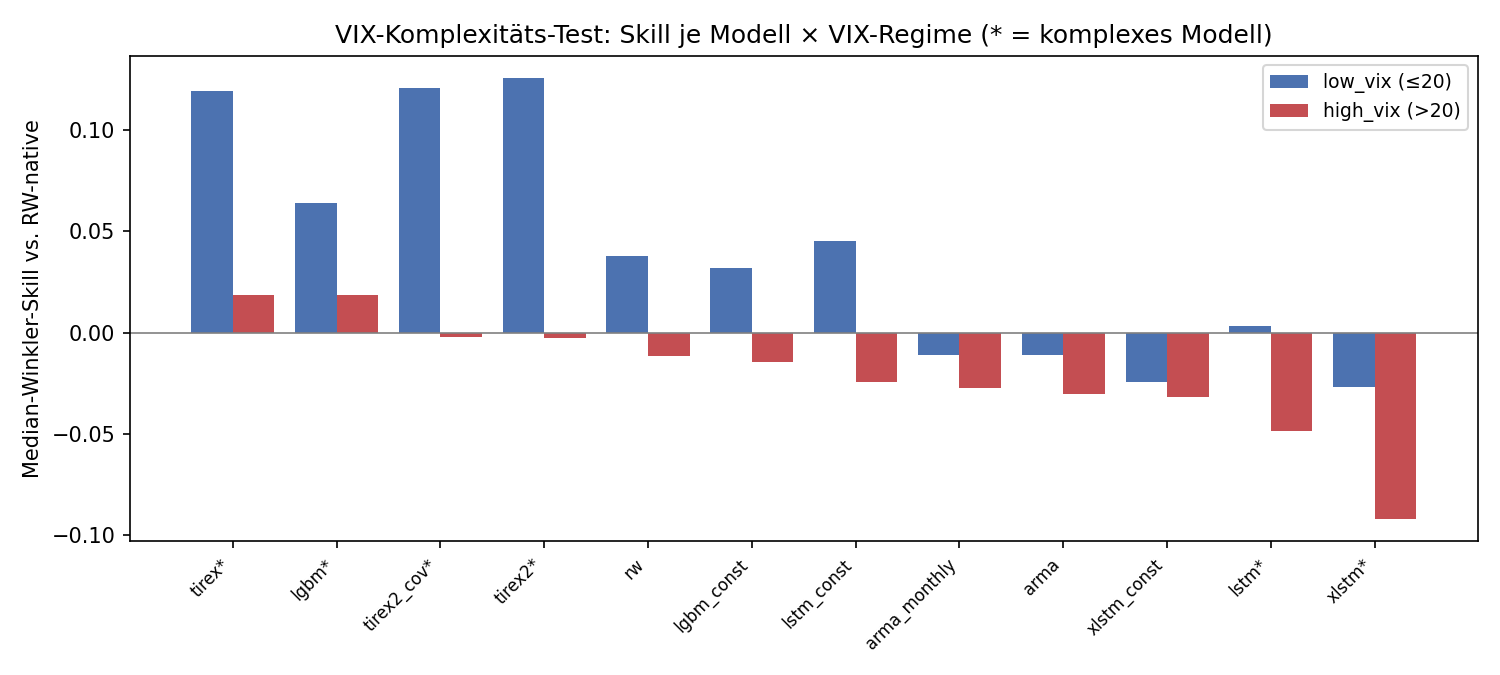
\includegraphics[width=0.8\textwidth]{figures/vix_complexity.png}
%   \caption{% TODO}
%   \label{fig:res_vix}
% \end{figure}
\begin{table}[t]
\centering
\caption{% TODO Caption. The eight largest cross-model contrasts by
         absolute effect size, out of 66. Effect as in
         \cref{tab:res_contrasts}; negative means A is better. None of
         the 66 contrasts is significant after FDR correction.}
\label{tab:res_xm}
\begin{tabular}{llrrrr}
\toprule
A & B & Effect & Share A better & Panel $t$ & median $q$ \\
\midrule
\texttt{tirex2}/ZS/\texttt{cqr\_static}    & \texttt{xlstm\_const}/L/\texttt{spci\_cqr} & $-0.116$ & 0.8 & $-3.55$ & 0.185 \\
\texttt{tirex2\_cov}/ZS/\texttt{native}    & \texttt{xlstm\_const}/L/\texttt{spci\_cqr} & $-0.111$ & 0.9 & $-4.16$ & 0.196 \\
\texttt{tirex}/ZS/\texttt{native}          & \texttt{xlstm\_const}/L/\texttt{spci\_cqr} & $-0.101$ & 1.0 & $-3.26$ & 0.263 \\
\texttt{lgbm}/G/\texttt{decay\_ocp\_cqr}   & \texttt{xlstm\_const}/L/\texttt{spci\_cqr} & $-0.090$ & 0.7 & $-2.92$ & 0.270 \\
\texttt{lstm\_const}/G/\texttt{agaci\_cqr} & \texttt{xlstm\_const}/L/\texttt{spci\_cqr} & $-0.080$ & 0.8 & $-2.43$ & 0.352 \\
\texttt{tirex2\_cov}/ZS/\texttt{native}    & \texttt{arma}/L/\texttt{dtaci\_cqr}        & $-0.075$ & 0.9 & $-3.09$ & 0.217 \\
\texttt{tirex2}/ZS/\texttt{cqr\_static}    & \texttt{lstm}/L/\texttt{pid\_cqr}          & $-0.074$ & 0.9 & $-3.09$ & 0.253 \\
\texttt{tirex2}/ZS/\texttt{cqr\_static}    & \texttt{arma}/L/\texttt{dtaci\_cqr}        & $-0.074$ & 0.9 & $-2.50$ & 0.255 \\
\bottomrule
\end{tabular}
\end{table}

%------------------------------------------------------------------------
\subsection{Economic evaluation}
\label{sec:res:econ}
%------------------------------------------------------------------------
% ERINNERUNG (7.7 + CLAUDE.md): dieser Block ist SEKUNDAER und darf nie
% zum Rangkriterium werden. Der erste Satz muss das sagen.
%
% WAS HIER STEHT:
%  1. Kapital-Proxy: der Median-Kapitalquotient ueber valide Kombis liegt
%     bei 0.669 (Spanne 0.551 bis 0.878). Also: valide, rekalibrierte
%     Intervalle sind im Median rund ein Drittel schmaler als der
%     breiteste valide Benchmark.
%  2. Der eigentlich interessante Befund: die Korrelation zwischen
%     Winkler-Skill und Kapitalquotient betraegt -0.711 (valide Kombis).
%     Hoher Skill geht also systematisch mit niedrigerem Kapitalbedarf
%     einher. -> Das ist die Bruecke von der statistischen zur
%     oekonomischen Metrik und rechtfertigt den Winkler-Score als
%     Rangkriterium nachtraeglich. Guter, zitierfaehiger Satz.
%  3. Der Kontrastbefund, der genauso wichtig ist: die Korrelation
%     zwischen Skill und dem Sharpe der Handelsregel betraegt nur -0.147,
%     also praktisch null und sogar leicht negativ.
%     -> Aussage: bessere Intervalle uebersetzen sich in Kapitaleffizienz,
%        aber NICHT in Handelsgewinne. Genau so schreiben. Das ist ein
%        ehrlicher Befund und schuetzt dich davor, dass jemand die
%        Arbeit als Trading-Paper missversteht.
%  4. Sharpe-Verteilung: Median 0.159, Spanne -0.607 bis 0.621, 68% der
%     validen Kombis haben positiven Sharpe. Der Active Share ist winzig
%     (die Regel handelt nur, wenn der Vormonatsspread ausserhalb des
%     Intervalls lag -- bei ~80% Coverage sind das per Konstruktion
%     wenige Monate). Beispielwerte: 0.003 bis 0.053.
%     -> Ein Satz: bei so wenigen aktiven Monaten ist der Sharpe
%        extrem verrauscht; die Zahl taugt nur zum Methodenvergleich,
%        nicht als Renditeaussage. Transaktionskosten sind ignoriert.
%  5. Die Top-Sharpe-Pakete sind NICHT die Top-Skill-Pakete
%     (lstm/L/pid_cqr 0.621 Sharpe bei nur 0.062 Skill; xlstm/GI/agaci
%     0.446 Sharpe bei NEGATIVEM Skill -0.111). Das ist die konkrete
%     Illustration von Punkt 3 -- unbedingt als Beispiel bringen.
%
% ZAHLEN (verifiziert, econ_results.csv gejoint mit validity_flag=True,
%   485 valide Kombis):
%   median_sharpe    : Median 0.159 | Min -0.607 | Max 0.621 | >0: 68%
%   median_cap_ratio : Median 0.669 | Min 0.551 | Max 0.878
%   corr(median_skill, median_sharpe)    = -0.147
%   corr(median_skill, median_cap_ratio) = -0.711
%   Top-Sharpe (valide): lstm/L/42/pid_cqr 0.621 (Skill 0.062)
%     | lstm_const/G/42/spci 0.609 (Skill 0.060)
%     | lstm_const/GF/43/sfogd 0.484 (Skill 0.016)
%     | lstm/L/42/dtaci 0.482 (Skill 0.057)
%     | xlstm/GI/44/agaci 0.446 (Skill -0.111)
%
% ZITATE: bcbs2019mar (Basel-Kontext, Proxy-Charakter betonen).
%
% [arXiv-Kuerzung]: 3 Saetze -- Kapitalquotient-Median, die beiden
%   Korrelationen, der "kein Trading-Signal"-Satz. Bei hartem Limit:
%   ganzes Unterkapitel in eine Fussnote.


%------------------------------------------------------------------------
\subsection{Robustness}
\label{sec:res:robustness}
%------------------------------------------------------------------------
% WAS HIER STEHT (vier Checks aus 7.8, je 2-3 Saetze):
%  1. KALIBRIERUNGSPOOL. Primaerfall rolling(36) gegen expanding,
%     rolling(24), rolling(48). Auf den 3180 gemeinsamen Zellen betraegt
%     die mittlere absolute Coverage-Differenz zu expanding 0.040
%     (Maximum 0.189), zu rolling24 0.021 (max 0.102), zu rolling48
%     0.016 (max 0.087).
%     -> Ehrlicher Satz: die Pool-Wahl ist NICHT vernachlaessigbar; im
%        Extremfall verschiebt sie die Coverage um fast 19 Prozentpunkte.
%        Die mittlere Coverage steigt mit laengerem Pool
%        (rolling24 0.813 < rolling48 0.820 < rolling 0.834
%        < expanding 0.843), was zur Ueberdeckungsdiagnose aus 8.1 passt:
%        laengere Pools erben alte, breitere Quantile.
%     -> Story-Report F8 nennt lstm/GI/cqr_rolling mit 8.9pp Differenz
%        rolling vs expanding als Extremfall.
%  2. EX-IRLAND. Spearman-Rangkorrelation der Rankings mit und ohne
%     Irland: rho = 0.939 ueber die 485 validen Kombis. Die Rangfolge
%     ist also stabil. ABER das Niveau nicht: der mittlere Skill faellt
%     um -0.021, und beim Spitzenreiter tirex2/ZS/cqr_static von 0.146
%     auf 0.103 (-0.043).
%     -> Zwei Saetze: (i) die Ordnung ist robust, (ii) rund ein Drittel
%        des absoluten Vorsprungs des Siegers stammt aus Irland allein.
%        Da IE mit Skill 0.231 das mit Abstand "leichteste" Land ist und
%        wegen der MNE-/Leprechaun-Verzerrung ohnehin unter Vorbehalt
%        steht, gehoert das prominent berichtet, nicht in eine Fussnote.
%     -> Am staerksten leidet lgbm/L: aci von 0.067 auf -0.027,
%        dtaci von 0.075 auf -0.009, agaci von 0.085 auf 0.009. Also
%        LightGBM im lokalen Regime lebt fast vollstaendig von Irland.
%  3. SEEDS. Nur NN-Modelle (588 Kombinationen ueber xlstm/lstm und ihre
%     const-Zwillinge). Die Seed-Spannweite des Skills betraegt im Median
%     0.043, im Mittel 0.051, maximal 0.315.
%     -> Die entscheidende Zahl: in 52% der NN-Kombinationen ist die
%        Seed-Spannweite GROESSER als der Betrag des Skills selbst.
%        Das heisst, fuer die Haelfte der NN-Ergebnisse ist die
%        Initialisierung ein groesserer Effekt als das Ergebnis.
%        Konsequenz nach der Seed-Disziplin aus 7.8: fuer diese Faelle
%        werden KEINE Rangaussagen getroffen. Diesen Satz explizit
%        schreiben -- er entwertet die schwachen xlstm-Zahlen nicht,
%        er ordnet sie richtig ein.
%     -> Konkreter Beleg aus dem Story-Report (F9): lstm/G/dtaci_cqr
%        mit Seed-Spanne 0.043 ueber dem Effekt.
%     -> Auch relevant fuer 8.3: xlstm/L/native (0.094) hat seed_span
%        0.102 -- die Spanne ist groesser als der Skill. Das beste
%        xlstm-Paket ist also seed-fragil. UNBEDINGT dazuschreiben.
%  4. BURN-IN (F11). Coverage in den ersten 36 Testmonaten gegen den Rest:
%     im Mittel ueber alle Methoden -0.011, also leichte UNTERdeckung
%     am Anfang. Der groesste Effekt liegt bei native (-0.066), gefolgt
%     von decay_ocp (-0.041), saocp (-0.037), cqr_static (-0.034).
%     Die adaptiven Online-Verfahren zeigen praktisch keinen Burn-in-
%     Effekt oder sogar das umgekehrte Vorzeichen (aci +0.015,
%     spci +0.012, dtaci +0.009).
%     -> Interpretation: der Effekt trifft genau die Methoden, die einen
%        gefuellten Kalibrierungspool brauchen, und nicht die, die online
%        nachregeln. Das ist konsistent und selbstlimitierend (mit
%        wachsendem Pool verschwindet er). Ehrlich, aber ohne Dramatik
%        berichten.
%     -> Ein Satz zur Doppelrolle: das HPO-Validierungsfenster dient
%        gleichzeitig als CP-Initialisierung. Das ist die eigentliche
%        Sorge hinter F11; die Messung zeigt, dass sie sich in einer
%        Anfangs-UNTERdeckung aeussert, nicht in kuenstlichem Optimismus.
%  5. Ein letzter Satz zur Laender-Konsistenz (F7): die mittlere paarweise
%     Kendall-Rangkorrelation der Kombinations-Rankings zwischen den
%     Laendern betraegt tau = 0.35. Die Rangfolge ist also nur schwach
%     laenderuebergreifend stabil -- ein weiteres Argument fuer die
%     zurueckhaltende Formulierung aus 8.8.
%
% ZAHLEN (verifiziert):
%   cells.csv, mittlere Coverage je pool_mode:
%     rolling24 0.8127 | rolling48 0.8204 | rolling 0.8341 | expanding 0.8432
%     Median-Skill: rolling24 +0.0003 | rolling48 +0.0142
%       | rolling -0.0126 | expanding -0.0111
%     paarweise |Differenz| auf 3180 gemeinsamen Zellen:
%       vs expanding  mean 0.0397  max 0.1890
%       vs rolling24  mean 0.0208  max 0.1024
%       vs rolling48  mean 0.0156  max 0.0866
%   robustness_ex_ie.csv (485 valide): mean d_skill -0.0210,
%     median -0.0176, Spearman rho(mit vs ohne IE) = 0.9392
%     Top-5 mit/ohne IE: tirex2/cqr_static 0.146->0.103 (-0.043)
%       | tirex2/decay_ocp 0.144->0.100 | tirex2/native 0.142->0.098
%       | tirex2_cov/native 0.141->0.097 | tirex2_cov/cqr_static
%       0.140->0.098
%     groesste Verschlechterung: lgbm/L/aci -0.094 | lgbm/L/dtaci -0.084
%       | lgbm/L/agaci -0.077 | arma_monthly/L/cqr_rolling -0.070
%   ranking_all.csv, seed_span ueber 588 NN-Kombis:
%     Median 0.0431 | Mittel 0.0514 | Max 0.3146
%     Anteil mit seed_span > |median_skill|: 0.52
%   cells.csv, cov_first36 minus cov_rest je Methode:
%     native -0.0664 | decay_ocp -0.0405 | saocp -0.0371 | cqr_static
%     -0.0336 | pid_tan -0.0100 | mondrian -0.0038 | agaci -0.0034
%     | pid_local -0.0025 | sfogd +0.0011 | pid +0.0039 | cqr_rolling
%     +0.0065 | dtaci +0.0090 | spci +0.0121 | aci +0.0146
%     Gesamtmittel: -0.0107
%   story_report.md F7: mittlere paarweise Kendall-tau zwischen
%     Laendern = 0.35
%
% ZITATE: keine neuen Pflichtzitate. Fuer die IE-/Leprechaun-Verzerrung
%   brauchst du EINE Quelle (CSO Irland "Modified GNI (GNI*)") -- steht
%   noch aus, siehe offener Punkt am Ende von evaluation.tex.
%
% [arXiv-Kuerzung]: 1 Absatz mit vier Stichpunkten inline. Die
%   Seed-Fragilitaet und der ex-IE-Niveaueffekt MUESSEN drin bleiben.


%------------------------------------------------------------------------
\subsection{Summary of findings}
\label{sec:res:summary}
%------------------------------------------------------------------------
% WAS HIER STEHT: 6-8 nummerierte Saetze, je einer pro Kernbefund, jeweils
% mit der tragenden Zahl. Das ist die Vorlage fuer Abstract und Conclusion
% -- schreib es so, dass du es dort fast woertlich wiederverwenden kannst.
%
% VORSCHLAG DER REIHENFOLGE (inhaltlich, du formulierst):
%  (1) Punktprognose: kein Modell schlaegt den Random Walk; das beste
%      MAE-Verhaeltnis ist 0.997 (tirex2), alle trainierten Modelle
%      liegen darueber.
%  (2) Kalibrierung: native Modellquantile sind systematisch ueberdeckend
%      (0.872 statt 0.80) und passieren das Gate nur in 13% der Faelle;
%      adaptive CP-Verfahren erreichen 96-100%.
%  (3) Intervallguete: das beste valide Paket ist ein Zero-Shot-
%      Foundation-Model (tirex2/ZS, Skill 0.14-0.15) vor dem besten
%      klassischen Ansatz (rw/L/aci_cqr, 0.085).
%  (4) Aber: kein einziger der 66 Cross-Model-Kontraste ist FDR-
%      signifikant (min. median-q 0.185), und die MCS schliesst fast
%      nichts aus. Die Rangfolge ist deskriptiv.
%  (5) Kovariaten: der ceteris-paribus-Kontrast ist null
%      (d_norm -0.00006, p 0.45); 17 makrooekonomische Kovariaten
%      liefern dem vortrainierten Modell keine Zusatzinformation.
%  (6) Pooling und Adaptivitaet: globales Pooling hilft den neuronalen
%      Modellen nicht (+0.017), Fine-Tuning schlaegt Laender-Embedding
%      klar (-0.054), und modelleigene adaptive Breiten sind im Median
%      schlechter als konstante (+0.020).
%  (7) xLSTM: die namensgebende Architektur ist die schwaechste Familie
%      (Median-Skill -0.047); das beste valide Paket ist seed-fragil
%      (Skill 0.094 bei Seed-Spanne 0.102).
%  (8) Regime: der Vorsprung der komplexen Modelle verschwindet im
%      Stress (Delta -0.077 von low- zu high-VIX; tirex2 von 0.125
%      auf -0.003).
%
% !! Wenn du (3) schreibst, muss die Entscheidung aus 8.3 Punkt 4
%    (cqr_static vs decay_ocp) hier konsistent durchgezogen sein.
%
% [arXiv-Kuerzung]: bleibt vollstaendig, das ist das Rueckgrat des Papers.


%========================================================================
%  ANSCHLUSS-KAPITEL
%------------------------------------------------------------------------
%  LIMITATIONS -- seit 2026-08-03 ein eigenes Kapitel:
%    sections/limitations.tex, eingebunden in main.tex nach diesem Kapitel.
%    Alle Punkte, die in diesem Results-Kapitel aufgeworfen werden, sind
%    dort in acht Unterkapiteln ausgeschrieben (9.1 Kontamination,
%    9.2 Gate/DQ, 9.3 Inferenz+Power, 9.4 Seeds, 9.5 Stichprobe/Panel,
%    9.6 Designentscheidungen, 9.7 Oekonomie, 9.8 Scope).
%    -> Neue Limitationen NICHT mehr hier sammeln, sondern direkt dort
%       einsortieren. Diese Liste ist bewusst geloescht, damit es keine
%       zweite Wahrheit gibt.
%    -> Aus diesem Kapitel sollten Vorwaertsverweise gesetzt werden:
%       8.1 Gate -> \cref{sec:lim:gate}
%       8.2 Punktprognose -> \cref{sec:lim:scope} (PT-Artefakt, DM-Test)
%       8.3 Ranking -> \cref{sec:lim:contamination} und \cref{sec:lim:seeds}
%       8.8 Cross-Model/MCS -> \cref{sec:lim:inference}
%       8.11 Robustheit -> \cref{sec:lim:sample} (ex-IE) und
%                          \cref{sec:lim:design} (Pool-Fenster)
%
%  Discussion -- noch nicht angelegt. Abgrenzung zu den Limitations:
%    dort steht, was die Befunde BEDEUTEN (warum Zero-Shot gewinnt, warum
%    xLSTM verliert, was das fuer die Praxis heisst), hier steht, wo sie
%    an ihre Grenzen stossen. Nicht vermischen.
%  Conclusion -- 1-2 Seiten, gestuetzt auf 8.12.
%========================================================================
